%!TEX root = ../main.tex
\newpage
\section{Coding}
\label{sec:code}
\vspace{-3mm}
In this section, we show that \DV\ is able to code at a very high level, both in terms of writing code from instructions and understanding existing code. \DV\ can handle a wide range of coding tasks, from coding challenges to real world applications, from low-level assembly to high-level frameworks, from simple data structures to complex programs such as games. \DV\ can also reason about code execution, simulate the effects of instructions, and explain the results in natural language. \DV\ can even execute pseudocode, which requires interpreting informal and vague expressions that are not valid in any programming language.

In its current state, we believe that \DV\ \textit{has a high proficiency in writing focused programs that only depend on existing public libraries, which favorably compares to the average software engineer's ability}. More importantly, it empowers both engineers and non-skilled users, as it makes it easy to write, edit, and understand programs. We also acknowledge that \DV\ is not perfect in coding yet, as it sometimes produces syntactically invalid or semantically incorrect code%(e.g., accuracy at $k=1$ is lower than $k=5$ in Table~\ref{tab:leetcode-results}), 
, especially for longer or more complex programs. \DV\ also sometimes fails to understand or follow the instructions, or produces code that does not match the intended functionality or style. 
With this acknowledgment, we also point out that \DV\ is able to improve its code by responding to both human feedback (e.g., by iteratively refining a plot in~\ref{fig:pyplot}) and compiler / terminal errors (examples in Section~\ref{sec:affordances}).
\vspace{-4mm}
\paragraph{Important Disclaimer:} As explained in the Introduction (see footnote 1 for example) our experiments were run on an early version of GPT-4. In particular all quantitative results will be different on the final version of GPT-4, although the general trends remain the same. We provide numbers here for illustration purpose only, the definitive benchmark results can be found in OpenAI's technical report \cite{gpt4}.
\vspace{-2mm}
%All the experiments in this section are based on an intermediate version of {\DV} in December, 2022. The model is further fine-tuned significantly for preciseness and safety, which might impact some of the evaluation results.}

%Coding requires reasoning, problem-solving, thinking abstractly, and comprehending complex ideas, as one has to design, implement, and debug algorithms that solve a given task.
%Coding is also a broad expert domain in itself, as it requires diverse and complex knowledge of syntax, semantics, logic, algorithms, data structures, and various programming paradigms and frameworks.
%Moreover, coding involves translating between abstract concepts and implicit requirements into very concrete instantiations. Finally, writing good code requires one to anticipate and keep track of the state of the program, and simulate the effects of instructions, which is a form of planning.
%In this section, we evaluate \DV's coding ability by instructing it to write various programs (from coding interviews to narrow subdomains such as data visualization or machine learning), and by testing its ability to understand and reason about existing code.

% Coding is the skill of creating and instructing computer programs to perform various tasks, such as designing websites, developing games, analyzing data, or controlling robots. Coding is critically important in the 21st century, as it enables people to create, communicate, and solve problems using digital technologies. Coding can be used for various purposes, such as developing websites, apps, games, animations, data analyses, artificial intelligence systems, robotics solutions, and more. 

% In this section, we demonstrate that \DV \ masters many aspects of coding at or beyond human capabilities.
% We begin with a sanity check, showing that \DV \ achieves superior performance in coding compared to any existing models on HumanEval dataset. We also observe that many of the errors \DV~ makes are due easily fixable by slight human twisting. 
\vspace{-1mm}
\subsection{From instructions to code}
\vspace{-1mm}
\subsubsection{Coding challenges}
\vspace{-2mm}
A common way to measure coding skill is to pose coding challenges that require implementing a specific functionality or algorithm.
We first benchmark \DV\ on HumanEval~\cite{humaneval}, a docstring-to-code dataset consisting of 164 coding problems that test various aspects of programming logic and proficiency.
As shown in Table~\ref{tab:humaneval}, \DV\ outperforms other LLMs, including \texttt{text-davinci-003} (the base model of ChatGPT) and other models trained specifically on code, \texttt{code-davinci-002}, and CODEGEN-16B~\cite{codegen}.
\vspace{-4mm}
\begin{table}[H]
\begin{center}
 \begin{tabular}{c|cccc}
\toprule
Model& \textbf{\DV} & \texttt{text-davinci-003} & Codex(\texttt{code-davinci-002}) & CODEGEN-16B \\
\midrule
\midrule
Accuracy& \textbf{82\%} & 65\% & 39\% & 30\% \\
\bottomrule
\end{tabular}
\end{center}
\vspace{-.6cm}
\caption{Zero-shot pass$@1$ accuracy comparison of different models on HumanEval}
\label{tab:humaneval}
\vspace{-3mm}
\end{table}


Although {\DV}'s accuracy shows a big jump compared to previous models, it could be that \DV\ has seen and memorized some (or all) of HumanEval during pre-training. To account for this possibility, we also evaluate it on LeetCode (\texttt{https://leetcode.com}), a popular platform for software engineering interviews, where new problems are constantly posted and updated.
We used LeetCode in Figure~\ref{fig:hired} in the introduction, where \DV\ passes all stages of mock interviews for major tech companies.
Here, to test on \emph{fresh} questions, we construct a benchmark of 100 LeetCode problems posted after October 8th, 2022, which is after \DV's pretraining period.
As seen in the example in Figure~\ref{fig:leetcode}, we paste the problem instructions into a prompt, ask \DV\ to write a python function, and use the official LeetCode online judge to check for correctness.
We present the results in Table~\ref{tab:leetcode-results}, where we compare \DV\ to other models and to human performance based on LeetCode contest results (users who fail all questions are not included, and thus this is a strong sample of humans).
We report both pass@1 and pass@5 accuracies, which measure whether the model produces a correct solution in the first or in the first five attempts, respectively. 
\DV\ significantly outperforms the other models, and is comparable to human performance (which we measure in Appendix~\ref{sec:leetcode-human}).
% Even though HumanEval is a well-established benchmark for assessing the programming skills of machine learning models, the data set has already been available on the internet since mid 2021, thus it is highly likely that \DV \ might have seen it during pre-training. To complement this evaluation, we also use a widely recognized training camp for human software engineers\textemdash LeetCode\footnote{https://leetcode.com/}. 

% \subsection{\DV~cracks technical interviews for software engineering roles}
% LeetCode hosts a comprehensive collection of coding questions on algorithm, data structure, database etc. According to the website, ``LeetCode is the golden standard for technical interviews. LeetCode problems are widely used during technical interviews at companies like Facebook, Hulu and Google.", which makes it an execellent benchmark for evaluating \DV's coding skills. LeetCode releases fresh questions via weekly contests. To rule out the memorization issue, we only select the 100 questions that are posted after October 8th, 2022 postdating the completion of \DV's pretraining using web data, to the best of our knowledge.
\vspace{-3mm}
\begin{table}[H]
\begin{center}
\begin{tabular}{l|c|c|c|c|c|c||c|c}
\toprule
  & \multicolumn{2}{c|}{Easy} &  \multicolumn{2}{c|}{Median} &  \multicolumn{2}{c||}{Hard} & \multicolumn{2}{c}{Overall}\\
\hline
pass@$k$  & $k=1$ & $k=5$ & $k=1$ & $k=5$ & $k=1$ & $k=5$ & $k=1$ & $k=5$\\
\hline
\textbf{\DV}              & \textbf{68.2} & \textbf{86.4} & \textbf{40.0} & \textbf{60.0} & \textbf{10.7} & \textbf{14.3} & \textbf{38.0} & \textbf{53.0}\\
\texttt{text-davinci-003} & 50.0 & 81.8 & 16.0 & 34.0 &  0.0 &  3.6 & 19.0 & 36.0\\
Codex (\texttt{code-davinci-002}) & 27.3 & 50.0 &  12.0 & 22.0 &  3.6 &  3.6 &  13.0 & 23.0\\
\hline
%\hline
Human (LeetCode users) & \multicolumn{2}{c|}{72.2} & \multicolumn{2}{c|}{37.7} & \multicolumn{2}{c||}{7.0} & \multicolumn{2}{c}{38.2} \\
\bottomrule
\end{tabular}
\end{center}
\vspace{-6mm}
\caption{Zero-shot pass@1 and pass@5 accuracies (\%) on LeetCode.}
\label{tab:leetcode-results}
\end{table}

%Qualitatively, we observe that \DV\ writes more comments than the other models, explaining its logic and assumptions, as well as using meaningful variable names. This suggests that \DV\ not only can produce syntactically and semantically correct code at a highly competitive level (as indicated by the previous results), but also code that is readable and clear, which are important aspects of good coding practice.

% We present in Table~\ref{tab:leetcode-results} that \DV \ achieves an accuracy surpassing Human average. Moreover, cwe contend that Human average is an \emph{overestimated} benchmark, as we exclude users that fail on all questions in each competition, and the competition is also inflated by the high performance of ACM teams who use LeetCode for international competition training. 
%Additionally, the accuracy of human coders on Hard problems is \emph{much higher}, but this may reflect survivor bias -- Only those who have high coding skills would try to solve these questions.  (Not true anymore)

% In the introduction, we also demonstrate that \DV \ can leverage its abilities on LeetCode to pass all stages of mock interview assessments in major tech companies in 10 minutes. \textbf{These results indicate that \DV \ has reached, or even surpassed human-level proficiency in solving LeetCode problems.}
%\DV\ demonstrates human-level performance in coding, one of the expert domains it can handle. It can accomplish various coding-related tasks, such as programming in different languages from natural language instructions, interpreting and running pseudo code with function calls and recursions, and debugging and modifying existing code. 
\begin{figure}[H]
\begin{AIbox}{\DV}
{\bf{Prompt:}}
\begin{minted}[breaklines, breaksymbol=, baselinestretch=1, fontsize=\tiny]{latex}
You are given a **0-indexed** `m x n` integer matrix `grid` and an integer `k`. You are currently at position `(0, 0)` and you want to reach position `(m - 1, n - 1)` moving only **down** or **right**.
Return *the number of paths where the sum of the elements on the path is divisible by* `k`. Since the answer may be very large, return it **modulo** `10**9 + 7`.
**Example 1:**
    Input: grid = [[5,2,4],[3,0,5],[0,7,2]], k = 3
    Output: 2
    Explanation: There are two paths where the sum of the elements on the path is divisible by k. The first path highlighted in red has a sum of 5 + 2 + 4 + 5 + 2 = 18 which is divisible by 3. The second path highlighted in blue has a sum of 5 + 3 + 0 + 5 + 2 = 15 which is divisible by 3.
**Example 2:**
    Input: grid = [[0,0]], k = 5
    Output: 1
    Explanation: The path highlighted in red has a sum of 0 + 0 = 0 which is divisible by 5.
**Constraints:**
-  `m == grid.length`
-  `n == grid[i].length`
-  `1 <= m, n <= 5 * 10**4`
-  `1 <= m * n <= 5 * 10**4`
-  `0 <= grid[i][j] <= 100`
-  `1 <= k <= 50`
**Hints:**
-  The actual numbers in grid do not matter. What matters are the remainders you get when you divide the numbers by k.
-  We can use dynamic programming to solve this problem. What can we use as states?
-  Let dp[i][j][value] represent the number of paths where the sum of the elements on the path has a remainder of value when divided by k.
\end{minted}


%›\begin{minipage}[t]{0.45\linewidth}
{\bf \DV:}
\vspace{-0.1cm}
\begin{minted}[breaklines, breaksymbol=, baselinestretch=1, fontsize=\tiny]{python}
class Solution(object):
    def numberOfPaths(self, grid, k):
        """
        :type grid: List[List[int]]
        :type k: int
        :rtype: int
        """
        # Define MOD as 10**9 + 7
        MOD = 10**9 + 7
        # Get the dimensions of the grid
        m = len(grid)
        n = len(grid[0])
        # Initialize a 3D dp array with all zeros
        # dp[i][j][value] represents the number of paths where the sum of the elements on the path has a remainder of value when divided by k
        dp = [[[0] * k for _ in range(n)] for _ in range(m)]
        # Base case: the first cell has only one path and its value is grid[0][0] % k
        dp[0][0][grid[0][0] % k] = 1
        # Loop through the grid
        for i in range(m):
            for j in range(n):
                # Skip the first cell
                if i == 0 and j == 0:
                    continue
                # Loop through all possible remainders
                for value in range(k):
                    # The number of paths to the current cell with the current remainder is equal to the sum of:
                    # - The number of paths to the top cell with the previous remainder
                    # - The number of paths to the left cell with the previous remainder
                    # The previous remainder is equal to the current remainder minus the current value, plus k if it is negative
                    prev = (value - grid[i][j]) % k
                    if i > 0:
                        dp[i][j][value] += dp[i - 1][j][prev]
                    if j > 0:
                        dp[i][j][value] += dp[i][j - 1][prev]
                    # Take the modulo to avoid overflow
                    dp[i][j][value] %= MOD
        # Return the number of paths to the bottom right cell with a remainder of 0
        return dp[m - 1][n - 1][0]
\end{minted}
\begin{comment}
\end{minipage}\hspace{0.02\linewidth}
\begin{minipage}[t]{0.53\linewidth}
{\bf \texttt{text-davinci-003}:}
\vspace{-0.2cm}
\begin{minted}[breaklines, breaksymbol=, baselinestretch=1, fontsize=\tiny]{python}
class Solution(object):
    def numberOfPaths(self, grid, k):
        """
        :type grid: List[List[int]]
        :type k: int
        :rtype: int
        """
        m, n = len(grid), len(grid[0])
        mod = 10**9 + 7
        dp = [[[0 for _ in range(k)] for _ in range(n)] for _ in range(m)]
        # Base cases
        # First row
        for j in range(n):
            dp[0][j][grid[0][j] % k] = 1
        # First column
        for i in range(1, m):
            dp[i][0][grid[i][0] % k] += dp[i - 1][0][grid[i][0] % k]
        # The rest
        for i in range(1, m):
            for j in range(1, n):
                for v in range(k):
                    dp[i][j][(v + grid[i][j]) % k] += dp[i - 1][j][v] + dp[i][j - 1][v]
        return dp[m - 1][n - 1][0] % mod
\end{minted}
%\end{minipage}%
%\begin{minipage}[t]{0.3\linewidth}
\vspace{-0.1cm}
{\bf Codex:}
\vspace{-0.2cm}
\begin{minted}[breaklines, breaksymbol=, baselinestretch=1, fontsize=\tiny]{python}
class Solution(object):
    def numberOfPaths(self, grid, k):
        """
        :type grid: List[List[int]]
        :type k: int
        :rtype: int
        """
        m = len(grid)
        n = len(grid[0])
        # dp[x][y][v] = number of paths from 0, 0 to x, y with sum of v
        dp = [[[0] * k for j in range(n)] for i in range(m)]
        dp[0][0][grid[0][0]%k] = 1
        for x in range(m):
            for y in range(n):
                for v in range(k):
                    if x < m-1:
                        dp[x+1][y][(v+grid[x+1][y])%k] += dp[x][y][v]
                    if y < n-1:
                        dp[x][y+1][(v+grid[x][y+1])%k] += dp[x][y][v]
        return dp[m-1][n-1][0]
\end{minted}
\end{minipage}
\end{comment}
\end{AIbox}
\caption{Solving a LeetCode problem using dynamic programming. \DV's solution also has better readability thanks to comprehensive commenting.}
\label{fig:leetcode}
\end{figure}

% One might still question the validity of the benchmarks in LeetCode or other sources, as they are very structured and some forms of the problems might already appear online. This could enable \DV \ to learn and replicate code patterns from the training data, rather than acquiring coding abilities that can generalize to new situations. How does \DV \ cope with more difficult and authentic coding tasks in real-world applications that are beyond the benchmarks? In this section, we further test \DV's coding ability with many challenging tasks, such as:
% \begin{enumerate}

% \item Zero-shot Programming from natural language instructions in real-world settings for diverse purposes, such as data visualization, deep learning with PyTorch, and GUI development. 
% \item Profound knowledge of coding, such as debugging, hacking and operation systems etc.  
% \item Interpreting and running code and \textbf{pseudo code} that involves complex logic and recursive functions. This requires the model to combine natural language interpretation with knowledge of the \textbf{innerworkings} of code.
% \end{enumerate}

% We argue that \DV \ also performs excellently on all these challenging tasks --  \textbf{These tasks not only significantly surpass the scope of existing models such as Codex, but also require significant domain knowledge and can take hours for a human expert to complete}. \DV \ can generate the correct answer in under a minute. We believe that \DV \ can fundamentally change the way we code in the future.

%\subsection{LeetCode}

%I left a place for you (to fill) above






% \subsection{\DV's extraordinary coding skills in real-world applications}

\subsubsection{Real world scenarios}
Coding challenges can evaluate the skills in algorithms and data structures. However, they often fail to capture the full complexity and diversity of real-world coding tasks, which requires specialized domain knowledge, creativity, and integration of multiple components and libraries, as well as the ability to change existing code. 
To assess \DV's ability to code in more realistic settings, we design end-to-end real-world coding challenges related to data visualization, \LaTeX\ coding, front-end development, and deep learning, each of which requires different specialized skills.
For each task, we provide \DV\ with high-level instructions, ask it to write the code in the appropriate language and framework. In a few cases, we also change the specification \emph{after} the code is written and ask for an update.

\paragraph{Data Visualization} %/ Data Science} 
In Figure~\ref{fig:pyplot}, we ask both \DV{} and ChatGPT to extract data from the \LaTeX\ code for Table~\ref{tab:leetcode-results} and produce a plot in Python based on a conversation with the user. Afterwards, we ask both models to perform various operations on the produced plots. While both models extract the data correctly (not a trivial task, since one must infer from the multicolumn that the Human row has the same value for $k=1$ and $k=5$), ChatGPT never produces the desired plot. In contrast, \DV{} responds appropriately to all user requests, manipulating the data into the right format and adapting the visualization. In Appendix~\ref{sec:imdb}, we include another example where \DV visualizes the IMDb dataset.
%by constructing a network graph, applying community detection algorithms as well as responding to customized requests from human.
\begin{figure}[H]
\centering
\begin{AIbox}{\DV}
\centering
\begin{tikzpicture}
% Define a 4x1 matrix of nodes, each containing an image
\matrix (m) [matrix of nodes, column sep=0cm, row sep=0.1cm] {
  %\includegraphics[width=0.6\linewidth, height=0.25\linewidth]{figures/DV3_plot_0.png} \\
  \includegraphics[width=0.6\linewidth, height=0.3\linewidth]{figures/DV3_plot_1.png} \\
  \includegraphics[width=0.6\linewidth, height=0.3\linewidth]{figures/DV3_plot_2.png} \\
  \includegraphics[width=0.6\linewidth, height=0.3\linewidth]{figures/DV3_plot_3.png} \\
};

%\draw [-triangle 90, arrowhead=15mm, bend left=30, thick] ([yshift=-0.5cm]m-1-1.east) to node [right, text width=0.35\linewidth, align=center] {\scriptsize \texttt{can you please move the legend outside of the plot, and have a single legend rather than two? Also, can we change the order to Codex, \texttt{text-davinci-003}, \DV, Human?}} ([yshift=0.5cm]m-2-1.east);
\node [left=0.2cm of m-1-1, text width=0.35\linewidth, align=left, anchor=east, yshift=-1] (start) 
{{\bf Prompt: }\\
{\scriptsize [in an interactive manner]}
\\
\hfill \break
\scriptsize\texttt{I will show you a LaTeX table, and we will come up with a way to visualize it better in a question and answer format
The table is showing the performance of different language models (and human users) in generating solutions to code challenges. Pass@1 means the first generation works, while Pass@5 means one out of 5 generation works...}};

% draw curved arrows from east to east with text boxes on the right
\draw [-triangle 90] (start) to ([xshift=0.1cm]m-1-1.west);

\draw [-triangle 90, bend right=30, thick] ([yshift=-2cm]m-1-1.west) to node [left, text width=0.35\linewidth, align=left, yshift=-1cm] 
{\scriptsize \texttt{Can you make both plots have the same range in the y axis? And the legend has each model name twice.}} ([yshift=-1cm]m-2-1.west);

\draw [-triangle 90, bend right=30, thick] ([yshift=-2cm]m-2-1.west) to node [left, text width=0.35\linewidth, align=left, yshift=-1cm] 
{\scriptsize \texttt{Is there a way to make the `Human' bar more distinctive, to separate it from the other 3?}} ([yshift=-1cm]m-3-1.west);
\end{tikzpicture}
\end{AIbox}
\caption{\DV visualizes data from a \LaTeX\ table (i.e., Table~\ref{tab:leetcode-results}). We point out that \DV also generates the format for this figure. We asked the model how to plot arrows connecting figures in \LaTeX\, and \DV produced a working Tikz snippet with the layout and arrows that we adopt here.}
\label{fig:pyplot}
\end{figure}


\begin{comment}

A function $f$ is called \emph{increasing} if $f(s) \leq f(t)$ holds for every $s \leq t$. Consider the formula:
\[
\lim_{x \to 0} \lim_{n \to \infty} \underbrace{ \begin{bmatrix} \sum_{i = 1}^n \left(f(nx) - \int_0^x \sin(nx) \, dx \right), & \frac{\left(x + \frac{2}{8}\right)^2 - 5}{\frac{4x-1/x^2}{n \oplus 3}}, \\ \vdots & \vdots \\ \frac{\partial f(x/n)}{\partial x} \cdot  \left(e^{-i \omega n x} + 3(x\#7) \right), & f^{-1} (x \bmod n) \end{bmatrix}  \times  \begin{bmatrix} 1 & 1 & \cdots & 1 \\ 1 & 1 & \cdots & 1 \end{bmatrix} }_{\textcolor{gray}{\text{this gives us a good impression about the function}}}
\]

\end{comment}


\begin{comment}
In Figure~\ref{fig:data-vis}, we give \DV{} a more open ended task, with a dataset specification. Again, during the course of conversation, \DV{} is able suggest and execute complex operations such as ``use a community detection algorithm to partition the nodes into subgroups'', and follow all user instructions. The final plot is interactive and responsive, and shows the clusters and patterns of the most successful and influential titles and people in the film industry, as intended by the task.

\begin{figure}[H]
\centering
\begin{AIbox}{\DV}
\begin{minipage}[t]{0.55\linewidth}
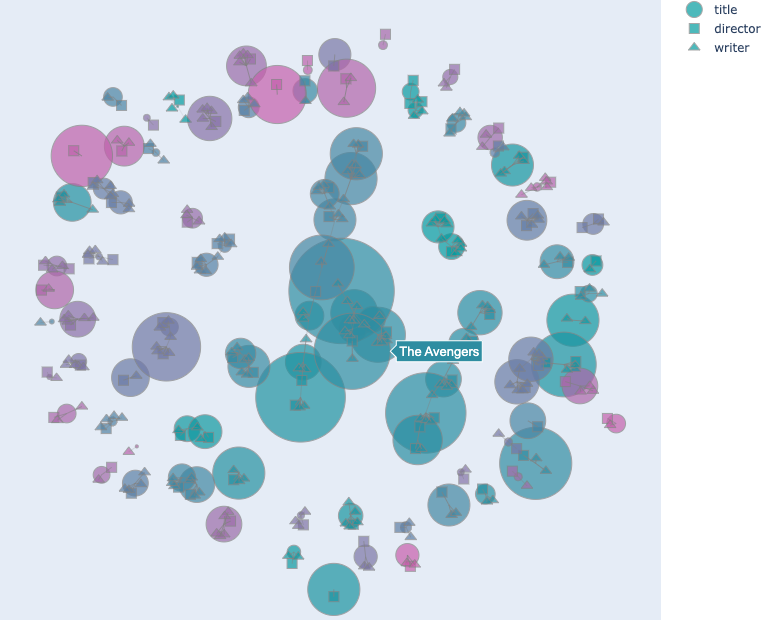
\includegraphics[width=\linewidth, height=0.9\linewidth]{figures/data_vis_1.png}
\caption*{}
\end{minipage}
\begin{minipage}[t]{0.45\linewidth}
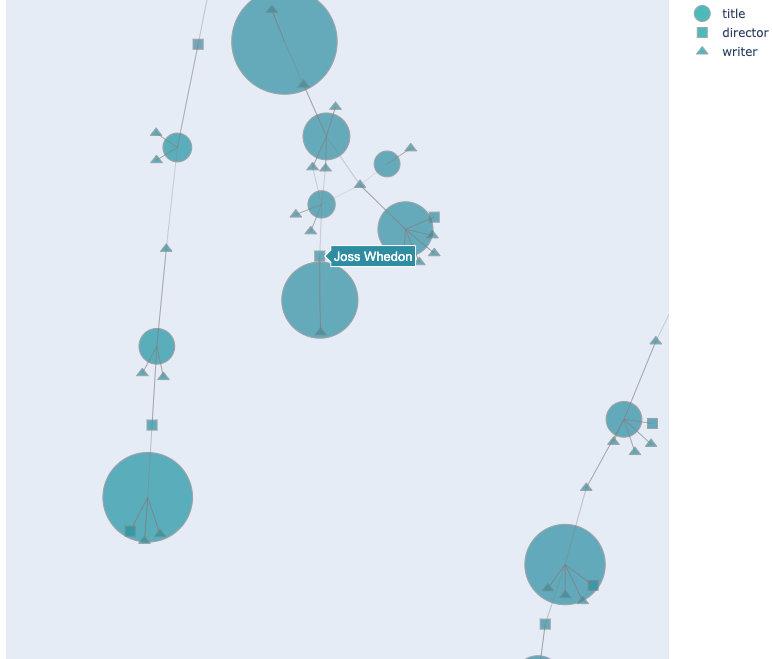
\includegraphics[trim={0 0 3cm 0}, clip, width=\linewidth, height=0.9\linewidth]{figures/data_vis_2.png}
\caption*{}
\end{minipage}
\tcbline
\vspace{-0.2cm}
\parbox[t]{\linewidth}{\tiny\begin{alltt}
Human: I am a Hollywood producer. We are starting a new project for an adventure movie in 2023, we are currently making critical decisions on the choices of directors and script writers. For this purpose, I have gathered some historical data ranging from 1888 to 2022. I have an IMDb dataset that consists of the 4 following files:\\

\#\# title.basics.tsv.gz - Contains the following information for titles:\\
> tconst (string) - alphanumeric unique identifier of the title\\
> titleType (string) – the type/format of the title (e.g., movie, short, tvseries, tvepisode, video, etc)\\
~~~\textbf{...}\\
\\
I'd like to know the best way to visualize this dataset with a single plot, so that our decision process can be made easier. Of course, our goal is to make this the best rated movie ever. What do you think?\\

AI: \hl{There are many possible ways to visualize this dataset, but one possible option is to use a network graph, where the nodes represent the titles, directors, writers, and actors, and the edges represent the relationships between them. The size and color of the nodes can be used to encode the average rating and the number of votes of the titles, or the popularity and reputation of the people. The thickness and opacity of the edges can be used to encode the frequency and strength of the collaborations between the nodes. This way, we can see the clusters and patterns of the most successful and influential titles and people in the film industry, and identify the potential candidates for our project.}\\
\\
Human: I like the idea, but since this dataset is quite large, a network graph might look messy. Is there anyway to simplify it?\\
\\
AI:\hl{ Yes, there are some possible ways to simplify the network graph. For example, we could:\\
- Filter out the titles and people that are not relevant to our genre or time period of interest.~~~\textbf{...}\\
- Aggregate the nodes that belong to the same group or category, and use a representative node to show their collective attributes.~~~\textbf{...}\\
- Use a hierarchical or modular layout to organize the nodes by their level of similarity or connection. For example, we could use a force-directed layout to place the nodes that are more closely related or frequently collaborated closer together, and use a community detection algorithm to partition the nodes into subgroups based on their network structure. ~~~\textbf{...}\\}
\\
Human: I think the last suggestion makes a lot sense to me. Could you please implement it for me in Python?\\
\\
AI:\hl{ Sure, here is a possible implementation of the network graph in Python, using the networkx, pandas, and plotly libraries. Note that this is not a fully functional code, and some parts are simplified or omitted for brevity. You will need to load and preprocess the dataset before running this code.~~~\textbf{...}}\\

Human: Wow, this looks amazing! Maybe just one slight suggestion, I am seeing the edges showing up in the legends. As there are many of them, they eat up a lot space. Can you tell me where in the code I can make them disappear from the legend?\\
\\
AI:\hl{ Sure, you can make the edges disappear from the legend by adding the argument showlegend=False to the go.Scatter trace that draws the edges.}
\\
Human: Great, that works perfectly! One last thing, could you please remove all the title names and crew names? They clutter the plot. Instead, can you make them appear only when I move mouse onto them?\\
\\
AI:\hl{ Sure, you can remove the text of title names by using the mode argument in the go.Scatter trace that draws the title nodes. For example, you can modify the code as follows:
~~~\textbf{...}
}
\end{alltt}}
\vspace{-0.5cm}
\end{AIbox}
\caption{}
\label{fig:data-vis}
\end{figure}
\end{comment}
\paragraph{Front-end / Game development}
In Figure~\ref{fig:games}, we ask \DV\ to write a 3D game in HTML with JavaScript, using a very high-level specification. \DV\ produces a working game in \textbf{zero-shot} fashion that meets all the requirements. In the 3D game, \DV{} is even able to interpret the meaning of ``defender avatar is trying to block the enemy'': the defender code has logic so that it positions itself between the player and enemy. In contrast, ChatGPT responds with ``I am an AI language model, I can provide you guidance on how to create a 3D game in HTML with JavaScript, but I am unable to write code or create a game myself.
Creating a 3D game in HTML with JavaScript requires a lot of programming knowledge and experience. It is not a task that can be completed quickly or easily. It would take a significant amount of time and effort to develop all the necessary features, such as 3D graphics, physics, user input, and AI...''. We give more examples for front-end (graphical user interface) and game development in Appendix~\ref{sec:code_appendix}. 

%

\begin{figure}[H]
\begin{AIbox}{\DV}
{\bf Prompt:}
\vspace{-0.3cm}
\begin{minted}[breaklines, breaksymbol=, baselinestretch=1, fontsize=\tiny]{html}
Can you write a 3D game in HTML with Javascript, I want:
-There are three avatars, each is a sphere.
-The player controls its avatar using arrow keys to move.
-The enemy avatar is trying to catch the player.
-The defender avatar is trying to block the enemy.
-There are also random obstacles as cubes spawned randomly at the beginning and moving randomly. The avatars cannot cross those cubes.
-The player moves on a 2D plane surrounded by walls that he cannot cross. The wall should cover the boundary of the entire plane. 
-Add physics to the environment using cannon.
-If the enemy catches the player, the game is over.
-Plot the trajectories of all the three avatars.
\end{minted}
%\vspace{-0.7cm}
\begin{subfigure}
\centering
\captionsetup{width=1\linewidth}
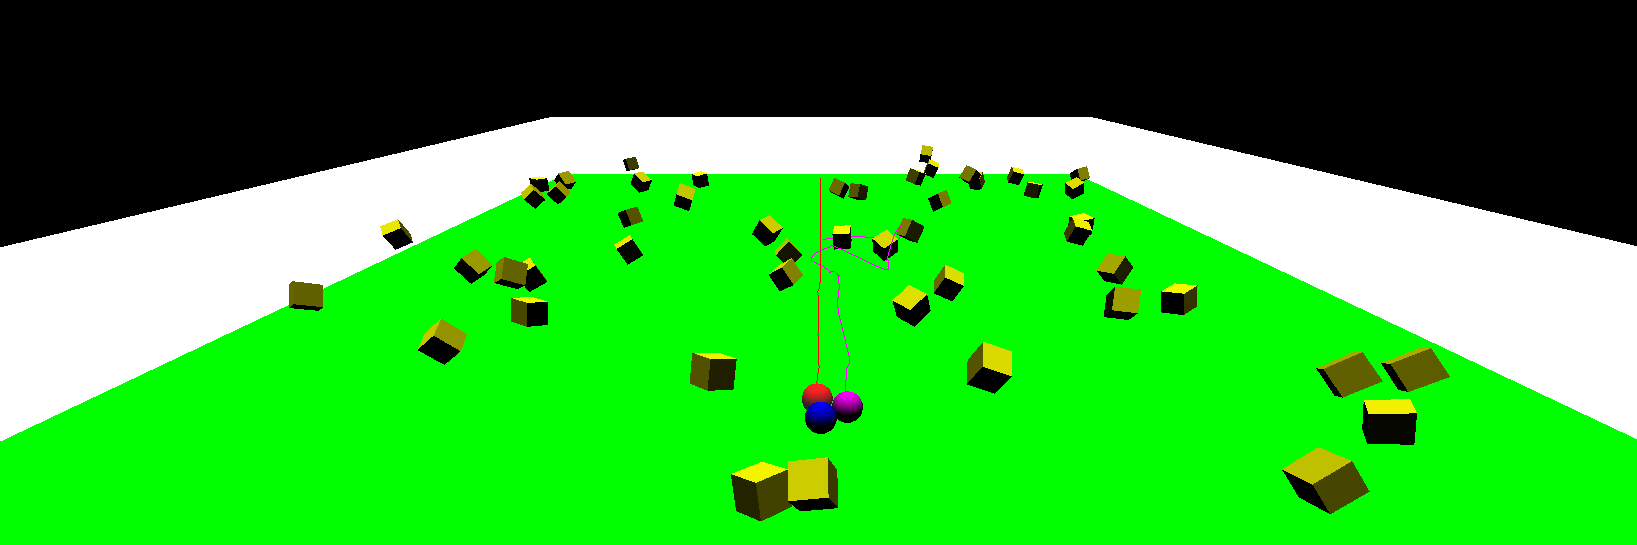
\includegraphics[width=1\linewidth]{figures/3d_game_run_1.png}
\caption*{\scriptsize {\bf Episode 1:} the player avatar (\textcolor{blue}{blue}) stands still. The enemy (\textcolor{red}{red}) rushes straight towards the player, while the defender (\textcolor{magenta}{magenta}) attempts to `body block' the enemy (see its curved trajectory in \textcolor{magenta}{magenta}).}
\end{subfigure}
\hfill
\begin{subfigure}
\centering
\captionsetup{width=1\linewidth}
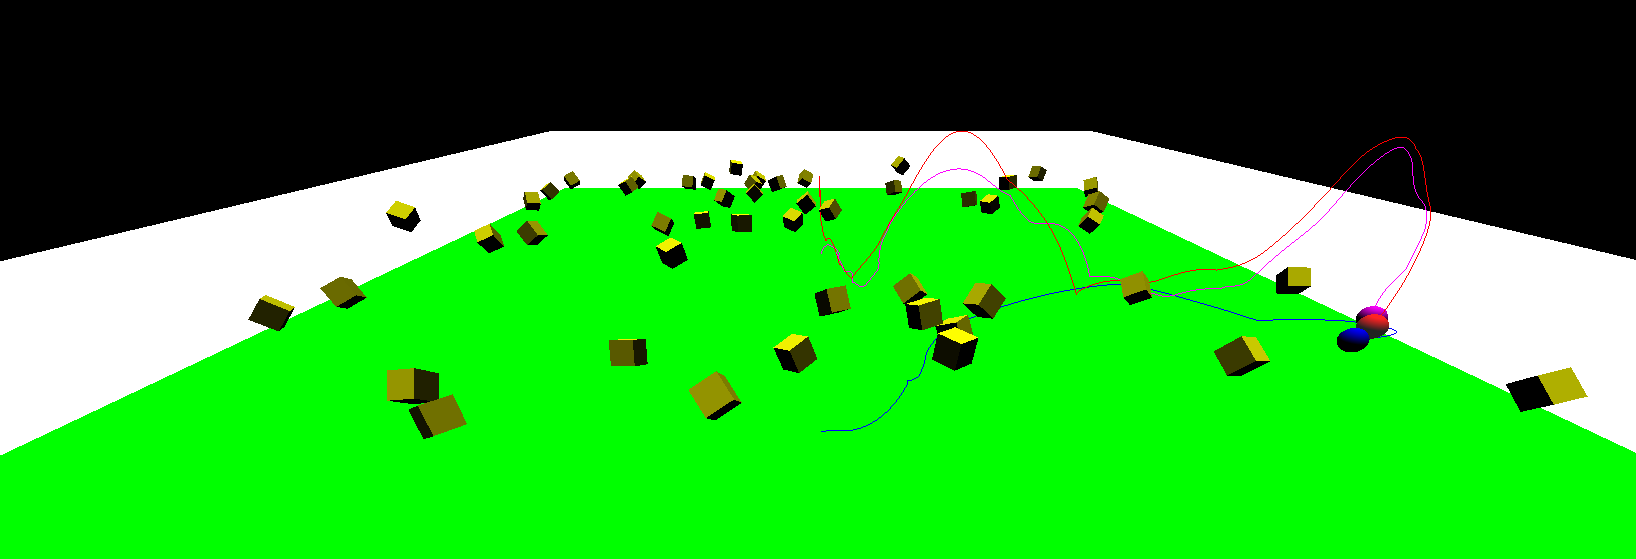
\includegraphics[width=1\linewidth]{figures/3d_game_run_2.png}
\caption*{\scriptsize {\bf Episode 2:} the player (\textcolor{blue}{blue}) wanders around. The enemy (\textcolor{red}{red}) attempts to close the gap but crashes into a cube and bounces into the air. Trying to obstruct, the defender (\textcolor{magenta}{magenta}) mimics its move to follow up into the air, but ends up failing. The enemy (\textcolor{red}{red}) catches the player (\textcolor{blue}{blue}) in the end.}
\end{subfigure}
\end{AIbox}
\caption{\DV~ develops a complex 3D HTML game in JavaScript.}
\label{fig:games}
\end{figure}


\paragraph{Deep Learning.}
Writing code for deep learning requires knowledge of mathematics, statistics, and familiarity with frameworks and libraries such as PyTorch, TensorFlow, Keras, etc. 
In Figure~\ref{fig:deeplearning} we ask both \DV\ and ChatGPT to write a custom optimizer module, a task that can be challenging and error-prone even for human deep learning experts. We give these models a natural language description, which includes a sequence of non-trivial operations such as applying SVD, truncating a matrix spectrally at the top-k and top-2k eigenvalues, normalizing the top-k truncated matrix using the F-norm of the top-2k truncated matrix, applying momentum and weight decay.
These instructions are not spelled out in complete detail, e.g., ``apply momentum on $G_k$'' requires ``deep learning common sense''.
It is important to note that this particular optimizer does not exist in the literature or on the internet, and thus the models cannot have it memorized, and must instead compose the concepts correctly in order to produce the code. 
% \begin{enumerate}[1)]
%     \item retrieve gradient from corresponding parameter
%     \item reshape gradients from 4d tensors into 2d matrices along a specific axis
%     \item apply SVD and then truncate spectrally at top-k and top-2k eigenvalues
%     \item normalize the top-k truncated matrix by the Frobenius norm of the top-2k truncated matrix
%     \item truncate the resulted matrix coordinate-wise to keep only the top $\alpha$-percentile of all coordinates
%     \item apply momentum on the resulted matrix (over past iterates)
%     \item update the parameter using the momentum estimate, along with weight decay
% \end{enumerate}



% TODO: Some closing sentence here


% \emph{We argue that \DV\ writes expert-level deep learning code, that is standardized and equipped with accurate comments for readability}, as we illustrate with an example of a novel and sophisticated optimizer in Pytorch that we design with \DV\.

% The \DV\ model shows impressive ability to infer the details of the optimizer logic and the Pytorch syntax from the prompt, and to generate code that is consistent and efficient. Remarkably, \DV\ understands what it means to `apply momentum' from the prompt. This is a non-trivial task that requires knowledge of the Pytorch syntax and the optimizer logic (i.e., momentum requires storing/reading the moving average into/from a separate state buffer). In comparison, ChatGPT does not know how to apply momentum at all, as it fails to realize the need for a state buffer and simply naively adds to the update the $W_k$ multiplied by the momentum coefficient (line labeled in red). This shows a difference between \DV\ and ChatGPT: While ChatGPT still relies on ``pattern matching'' to simply multiply momentum to the update, \DV\ understands what is momentum and translates the domain knowledge to accurate code. 



\begin{figure}[H]
\begin{AIbox}{\DV~vs ChatGPT}
{\bf Prompt:}
\begin{minted}[breaklines, breaksymbol=, baselinestretch=1, fontsize=\tiny]{html}
I want to write a customized optimizer in pytorch, the optimizer should do:
1. the parameters for the optimizer is learning rate, momentum ,weigth decay, d_dim, k and factor alpha
2. the optimizer goes through each parameter in the network, and then
-- Get the gradient of this parameter, reshape it to 2D by looping through the dimensions, and keeping the dimension whose actual dimension (shape) is equal to d_dim, do an SVD decomposition of the parameter so W = U\Sigma V. 
-- Keep the top k singular vectors of W, so we get a new matrix W_k = U \Sigma_k V. 
-- Keep the top 2k singular vectors of W, so we get a new matrix W_{2k} = U \Sigma_{2k} V. 
-- Normalize W_k according to the momentum of the F-norm of W_{2k}.
-- Truncate each coordinate of W_k to the top alpha  percentile of all the coordinates, in absolute value.
-- Apply momentum on W_k, and then update the network parameters using this momentum.
-- Apply weight decay.
\end{minted}
\begin{minipage}[t]{0.5\linewidth}
{\bf \DV:}
\begin{minted}[breaklines, breaksymbol=, baselinestretch=1, fontsize=\tiny, highlightlines={20-23}, highlightcolor=aigold]{python}
def step(self):
    for group in self.param_groups:
        for p in group['params']:
            if p.grad is None:
                continue
            grad = p.grad.data
            # reshape grad to 2D
            grad_2d = grad.reshape(-1, group['d_dim'])
            # SVD decomposition
            U, S, V = torch.svd(grad_2d)
            # keep top k singular vectors
            G_k = U[:, :group['k']] @ torch.diag(S[:group['k']]) @ V[:, :group['k']].T
            # keep top 2k singular vectors
            G_2k = U[:, :2*group['k']] @ torch.diag(S[:2*group['k']]) @ V[:, :2*group['k']].T
            # normalize G_k 
            G_k /= torch.norm(G_2k, p=2)
            # truncate G_k 
            threshold = torch.quantile(torch.abs(G_k), group['alpha'])
            G_k[torch.abs(G_k) < threshold] = 0
            # apply momentum
            if 'momentum_buffer' not in group:
                group['momentum_buffer'] = torch.zeros_like(G_k)
            group['momentum_buffer'] = group['momentum'] * group['momentum_buffer'] + G_k 
            # update parameters
            p.data.add_(-group['lr'] * group['momentum_buffer'])
            # apply weight decay
            if group['weight_decay'] != 0:
                p.data.add_(-group['weight_decay'] * group['lr'], p.data)
\end{minted}
\end{minipage}
\begin{minipage}[t]{0.5\linewidth}
{\bf ChatGPT:}
\begin{minted}[breaklines, breaksymbol=, baselinestretch=1, fontsize=\tiny, highlightlines={24}, highlightcolor=aired]{python}
def step(self):
    for group in self.param_groups:
        for p in group['params']:
            if p.grad is None:
                continue
            grad = p.grad.data
            grad = grad.reshape(-1, grad.shape[-1]) # reshape to 2D
            
            # SVD decomposition
            u, s, v = torch.svd(grad)
            
            # Keep top k and 2k singular vectors
            k = group['k']
            u_k = u[:,:k]
            s_k = s[:k]
            v_k = v[:,:k]
            u_2k = u[:,:2*k]
            s_2k = s[:2*k]
            v_2k = v[:,:2*k]
            
            # Normalize according to momentum of F-norm of G_2k
            grad_k = u_k @ torch.diag(s_k) @ v_k.t()
            norm_2k = s_2k.norm()
            grad_k = grad_k * group['momentum'] / norm_2k
            
            # Truncate to top alpha percentile
            alpha = group['alpha']
            percentile = grad_k.abs().flatten().kthvalue(int(alpha * grad_k.numel()))
            grad_k[grad_k.abs() < percentile] = 0
            
            # Apply weight decay
            p.data.add_(-group['lr'], grad_k + group['weight_decay'] * p.data)
\end{minted}
\end{minipage}
\end{AIbox}
\caption{\DV~vs ChatGPT at implementing a customized Pytorch optimizer module. We highlight the \fcolorbox{aigold}{aigold}{astuteness} of \DV vs the \fcolorbox{aired}{aired}{mistake} by ChatGPT at `applying momentum'. }
\label{fig:deeplearning}
\end{figure}


While both models produce syntactically valid code, only \DV's code is semantically correct and matches the instructions. In contrast, ChatGPT makes a mistake at applying momentum (highlighted in red), a non-trivial task that requires storing and reading a moving average into and from a separate state buffer.


\paragraph{Interfacing with \LaTeX.} Writing in \LaTeX\ is an important exercise for computer scientists and mathematicians but has a non-trivial learning curve. Even experts make irritating errors that take hours to fix on a daily basis due to its strict grammar and the lack of a good debugger. We show that {\DV} can utilize its master-level \LaTeX\ coding skill to greatly simplify the process, with the potential of serving as a new generation of \LaTeX\ compilers that can handle imprecise natural language descriptions. In~Figure~\ref{fig:code-LaTeX}, we ask {\DV} to transfer a snippet of written in a semi-rigorous (buggy) \LaTeX\ code mixed with natural language into accurate \LaTeX\ commands that compiles and is faithful in one shot. In constrast, ChatGPT generates a snippet that does not compile due to mistakes at using `\#' and `\textbackslash{color}' etc.

\begin{figure}[H]
\begin{AIbox}{\DV vs ChatGPT}
{\bf Prompt:}
\begin{minted}[breaklines, breaksymbol=, baselinestretch=1, fontsize=\tiny]{html}
A function f is called {increasing}_{emphasize!} if f(s) <= f(t) holds for every s <= t. Consider the formula:
limit_{x goes to 0} {limit when n approaches infinite} underscore{ 
\matrix[ [ sum of i from 1 to n (f(nx) - integral from 0 to x sin(nx) dx ),  
((x + 2/8)^2 - 5)/((4x-1/x^2) /(n xor 3)), \\ , ..., partial f(x/n)
over partial x * (e^{-i*omega n x} + 3(x#7) ) , f inverse of (x mod n) ]]
multiply \matrix{1, 1, ..., 1 \\ 1, 1, ..., 1} }
{grey_color{this gives us a good impression about the function}}

Convert the above paragraph to LaTeX.
\end{minted}
\begin{comment}
\begin{minted}[breaklines, breaksymbol=, baselinestretch=1, fontsize=\scriptsize]{LaTeX}
A function $f$ is called \emph{increasing} if $f(s) \leq f(t)$ holds for every $s \leq t$. Consider the formula:
\[
\lim_{x \to 0} \lim_{n \to \infty} \underbrace{ \begin{bmatrix} \sum_{i = 1}^n \left(f(nx) - \int_0^x \sin(nx) \, dx \right), & \frac{\left(x + \frac{2}{8}\right)^2 - 5}{\frac{4x-1/x^2}{n \oplus 3}}, \\ \vdots & \vdots \\ \frac{\partial f(x/n)}{\partial x} \cdot  \left(e^{-i \omega n x} + 3(x\#7) \right), & f^{-1} (x \bmod n) \end{bmatrix}  \times  \begin{bmatrix} 1 & 1 & \cdots & 1 \\ 1 & 1 & \cdots & 1 \end{bmatrix} }_{\textcolor{gray}{\text{this gives us a good impression about the function}}}
\end{minted}
\end{comment}
\parbox[t]{\linewidth}{{\bf \DV:}\\\scriptsize
A function $f$ is called \emph{increasing} if $f(s) \leq f(t)$ holds for every $s \leq t$. Consider the formula:
\[
\lim_{x \to 0} \lim_{n \to \infty} \underbrace{ \begin{bmatrix} \sum_{i = 1}^n \left(f(nx) - \int_0^x \sin(nx) \, dx \right), & \frac{\left(x + \frac{2}{8}\right)^2 - 5}{\frac{4x-1/x^2}{n \oplus 3}}, \\ \vdots & \vdots \\ \frac{\partial f(x/n)}{\partial x} \cdot  \left(e^{-i \omega n x} + 3(x\#7) \right), & f^{-1} (x \bmod n) \end{bmatrix}  \times  \begin{bmatrix} 1 & 1 & \cdots & 1 \\ 1 & 1 & \cdots & 1 \end{bmatrix} }_{\textcolor{gray}{\text{this gives us a good impression about the function}}}
\]}\\
{\bf ChatGPT:}
\begin{minted}[breaklines, breaksymbol=, baselinestretch=1, fontsize=\scriptsize]{html}
A function $f$ is called {\em increasing} if $f(s) \leq f(t)$ holds for every $s \leq t$. Consider the formula:
$$\lim_{x \to 0} \lim_{n \to \infty} \begin{bmatrix} \sum\limits_{i=1}^{n} (f(nx) - \int\limits_0^x \sin(nx),dx), \ \frac{(\frac{x}{2} + \frac{1}{8})^2 - 5}{\frac{4x - \frac{1}{x^2}}{n \operatorname{xor} 3}}, \ \vdots, \ \frac{\partial f(x/n)}{\partial x} \cdot (e^{-i\omega n x} + 3(x#7)), \ f^{-1}(x \bmod n) \end{bmatrix} \cdot \begin{bmatrix} 1 \ 1 \ \vdots \ 1 \end{bmatrix}$$
{\color{grey}This gives us a good impression about the function.} \]
\end{minted}
\end{AIbox}
\caption{\DV translates semi-rigorous typesetting instructions into a working \LaTeX\ snippet. For \DV we present the final graphic, while ChatGPT's generation fails to compile. }
\label{fig:code-LaTeX}
\end{figure}

\subsection{Understanding existing code}
The previous examples have shown that \DV\ can write code from instructions, even when the instructions are vague, incomplete, or require domain knowledge. They also showed that \DV\ could respond to follow-up requests, modifying its own code according to instructions.
However, another important aspect of coding is the ability to understand and reason about existing code, written by others, which might be complex, obscure, or poorly documented. 
To test this we pose various questions that require reading, interpreting, or executing code written in different languages and paradigms.

\paragraph{Reverse-engineering assembly code.}
Reverse engineering is an essential test for software security which amounts to search for useful information in a executable program written in a machine-readable (i.e., binary) representation of CPU instructions. It is a challenging task that requires understanding the syntax, semantics, and conventions of assembly language, as well as the architecture and behavior of the processor and the operating system. 

We task \DV\ with performing penetration testing on a binary executable file (code was written in C) that requires a password to run. We do this via a chat format, where \DV\ tells the user which commands to run, and the user responds with the results. We also show in Section~\ref{sec:affordances} that \DV\ is able to run a shell independently, but this chat mode also provided the benefit of it explaining every step. \DV\ checks the file format and metadata, disassembles the code with tools like ``objdump'' and ``radare2'', debugs the code with ``gdb'' and ``ltrace'', and reverse engineers it with techniques like patching, hooking, and decompiling. During this process, \DV\ figures out that from the assembly code that the password is compared to a hash value derived from a simple mathematical formula. \DV\ then writes a python program that tries different combinations of numbers until it finds one that matches the hash value, cracking the password (an abbreviated log is presented in Appendix~\ref{appendix:reverse-engine}). ChatGPT refuses to do it on the grounds of it being illegal and unethical, even though reverse engineering is a common practice to \emph{ensure} software security. Moreover, \DV exhibits all-around proficiency in utilizing existing tools also beyond programming, which we will discuss in details in Section~\ref{sec:affordances}.


\paragraph{Reasoning about code execution.}
In the example in Figure~\ref{fig:code-memory-align}, we ask \DV and ChatGPT to predict and explain the output of a C program that prints the size of two structures. \DV correctly explains that the output may vary depending on the alignment rule used by the compiler, and gives an example of a possible output with 4-byte alignment. ChatGPT ignores the alignment issue and gives a wrong output, and also makes a false statement about the order of the members not affecting the size of the structure.

\begin{figure}[H]
\begin{AIbox}{\DV~vs ChatGPT}

{\bf Prompt:}  


 \begin{minted}[breaklines, breaksymbol=, baselinestretch=1, fontsize=\scriptsize]{cpp}
struct mystruct_A {  char a; int b; char c; } x;
struct mystruct_B {  int b;  char a; char c; } y;
    
#include <stdio.h>
int main(void) {
    printf("Size of x: %zu bytes\n", sizeof(x)); 
    printf("Size of y: %zu bytes\n", sizeof(y));
    return 0;
}
    
Possible Output:
\end{minted}   

\parbox[t]{0.53\linewidth}{{\bf \DV:} 
\tiny
\begin{alltt}
There are different ways to implement and align structures in memory, so the exact output may vary depending on the compiler, platform, and options used. However, one possible output is:\\

Size of x: 12 bytes\\
Size of y: 8 bytes\\

This output assumes that the compiler uses 4-byte alignment for structures, meaning that each structure member starts at an offset that is a multiple of 4 bytes from the beginning of the structure. This may result in some padding bytes being inserted between or after the members to maintain alignment. For example, 
\fcolorbox{aigold}{aigold}{in x, there may be 3 padding bytes after a and 3 padding bytes after c,}
\fcolorbox{aigold}{aigold}{while in y, there may be no padding at all.} 
The size of a structure is the sum of the sizes of its members plus any padding bytes.
\end{alltt}
}\hspace{0.02\linewidth}%
\parbox[t]{0.45\linewidth}{{\bf ChatGPT:}
\tiny
\begin{alltt}
Size of x: 8 bytes\\
Size of y: 8 bytes\\

The output of this code would be the size of the two structures in bytes. The size of a structure in C is the sum of the sizes of all of its members. In this case, the size of mystruct\textunderscore A is the size of a char plus the size of an int plus the size of another char, which is \fcolorbox{aired}{aired}{1 + 4 + 1 = 8} bytes. \\
\\
Similarly, the size of mystruct\textunderscore B is also 8 bytes. This means that both structures will be allocated the same amount of memory. \\
\\
\fcolorbox{aired}{aired}{Note that the order in which the members are}
\fcolorbox{aired}{aired}{declared in the structure does not affect its}
\fcolorbox{aired}{aired}{size.}
\end{alltt}
}
\end{AIbox}
\caption{\DV vs ChatGPT on the~memory alignment rule of C/C\texttt{++}. \DV's insightful comments are labeled in \fcolorbox{aigold}{aigold}{gold} and ChatGPT's Mistakes are labeled in \fcolorbox{aired}{aired}{red}.}
\label{fig:code-memory-align}
\end{figure}


\paragraph{Executing Python code} The ultimate test of understanding the existing code is to ask the model to directly execute it. 
In Figure~\ref{figure:pseudo1}, we see that \DV{} is able to execute non-trivial Python code. It has to keep track of several variables (including a nested loop and a dictionary) and deal with recursion. It explains the execution in detail by writing intermediate steps and comments. It is important to note that \DV{} is not running the code on a Python interpreter, but rather simulating the code in natural language. This requires a high level of understanding and reasoning about the code, as well as the ability to communicate the results clearly. In contrast, ChatGPT states (incorrectly) that ``The result of DP(3, 4) is not specified in the given code'', and later on that ``It is not clear from the code what the expected output of the function is, as the specific problem that the function is solving is not provided.'' ChatGPT does not simulate the full execution, but states which functions will be called. %incorrectly including ``DP(0, 4)'' (i.e., it does not interpret the ``range'' function in python correctly).
\begin{figure}[H]
\begin{AIbox}{\DV vs ChatGPT}
\begin{minipage}[t]{0.15\linewidth}
{\bf Prompt:}
\end{minipage}
\begin{minipage}[t]{0.8\linewidth}
{\tiny
I have the following python code:}
\vspace{-0.1cm}
\begin{minted}[breaklines, breaksymbol=, baselinestretch=1, fontsize=\tiny]{python}
def to_str(i, j):
    return str(i) + "," + str(j)
dict = {}
def DP(i, j):
    if i <= 0 or j <= 0:
        dict[to_str(i, j)] = abs(4 * j - 3 * i) 
    elif to_str(i, j) not in dict.keys():
        arr = []
        for ir in range(i):
            for jr in range(j):
                arr.append(DP(ir, jr))
        dict[to_str(i, j)] = max(arr)
    return dict[to_str(i, j)]
\end{minted}
\vspace{-0.5cm}
{\tiny What is the result of DP(3, 4)? Write down the execution with intermediate steps.}\\
\end{minipage}
\vspace{-0.5cm}
% - dict["1,2"] = max(arr2) = 4, dict = {"0,0": 0, "0,1": 4, "0,2": 8, "0,3": 12, "1,0": 3, "1,1": 0, "1,2": 4}, arr = [0, 4, 8, 12, 3, 0, 4]

{\bf\DV:}
\vspace{-0.1cm}
\begin{minted}[breaklines, breaksymbol=,  fontsize=\tiny]{html}
DP(3, 4):
- i > 0 and j > 0, so we don't return from the first if statement
- to_str(3, 4) is not in dict, so we enter the second if statement
- arr = []
- We loop through ir from 0 to 2, and jr from 0 to 3
  - to_str(0, 0)  is not in dict, so DP(0, 0) returns abs(4 * 0 - 3 * 0) = 0, dict =  {"0,0": 0}, arr = [0]
  - to_str(0, 1)  is not in dict, so DP(0, 1) returns abs(4 * 1 - 3 * 0) = 4, dict =  {"0,0": 0, "0,1": 4}, arr = [0, 4]
  - to_str(0, 2)  is not in dict, so DP(0, 2) returns abs(4 * 2 - 3 * 0) = 8, dict =  {"0,0": 0, "0,1": 4, "0,2": 8}, arr = [0, 4, 8]
  - to_str(0, 3)  is not in dict, so DP(0, 3) returns abs(4 * 3 - 3 * 0) = 12, dict =  {"0,0": 0, "0,1": 4, "0,2": 8, "0,3": 12}, arr = [0, 4, 8, 12]
  - to_str(1, 0)  is not in dict, so DP(1, 0) returns abs(4 * 0 - 3 * 1) = 3, dict =  {"0,0": 0, "0,1": 4, "0,2": 8, "0,3": 12, "1,0": 3}, arr = [0, 4, 8, 12, 3]
  - to_str(1, 1)  is not in dict, so DP(1, 1) enters  the second if statement, arr1 = [] 
 - We loop through  ir from 0 to 0, and jr from 0 to 0
   - to_str(0, 0) is in dict, so DP(0, 0) returns 0, arr1 = [0]
 - dict["1,1"] = max(arr1) = 0, dict =  {"0,0": 0, "0,1": 4, "0,2": 8, "0,3": 12, "1,0": 3, "1,1": 0}, arr = [0, 4, 8, 12, 3, 0]
 - Continuing with the outer loop, to_str(1, 2) is not in dict, so DP(1, 2) enters the second if statement, arr2 = []
 - We loop through ir from 0 to 0, and jr from 0 to 1
   - to_str(0, 0) is in dict, so DP(0, 0) returns 0, arr2 = [0]
   - to_str(0, 1) is in dict, so DP(0, 1) returns 4, arr2 = [0, 4]
... (we skip some steps generated by the model here due to space constraints)
 - Continuing with the outer loop, to_str(2, 3) is not in dict, so DP(2, 3) enters the second if statement, arr6 = []
 - We loop through ir from 0 to 1, and jr from 0 to 2
   - to_str(0, 0) is in dict, so DP(0, 0) returns 0, arr6 = [0]
   - to_str(0, 1) is in dict, so DP(0, 1) returns 4, arr6 = [0, 4]
   - to_str(0, 2) is in dict, so DP(0, 2) returns 8, arr6 = [0, 4, 8]
   - to_str(1, 0) is in dict, so DP(1, 0) returns 3, arr6 = [0, 4, 8, 3]
   - to_str(1, 1) is in dict, so DP(1, 1) returns 0, arr6 = [0, 4, 8, 3, 0]
   - to_str(1, 2) is in dict, so DP(1, 2) returns 4, arr6 = [0, 4, 8, 3, 0, 4]
 - dict["2,3"] = max(arr6) = 8, dict =  {"0,0": 0, "0,1": 4, "0,2": 8, "0,3": 12, "1,0": 3, "1,1": 0, "1,2": 4, "1,3": 8, "2,0": 6, "2,1": 3, "2,2": 4, "2,3": 8}, arr = [0, 4, 8, 12, 3, 0, 4, 8, 6, 3, 4, 8]
- dict["3,4"] = max(arr) = 12
- DP(3, 4) returns 12
\end{minted}
{\bf ChatGPT:}\\
\vspace{-0.3cm}
\parbox[t]{\linewidth}{\tiny\begin{alltt}
The result of DP(3, 4) is not specified in the given code. The function DP(i, j) is a dynamic programming function that uses a dictionary to store the result of previously computed values. The function first checks if the input values i and j are less than or equal to 0, if so it assigns the value of abs(4 * j - 3 * i) to the key to\textsubscript{str}(i, j) in the dictionary. If the key to\textsubscript{str}(i, j) does not exist in the dictionary, the function creates an empty array called arr and then uses nested for loops to append the result of DP(ir, jr) to the array for all possible values of ir and jr, where ir ranges from 0 to i and jr ranges from 0 to j. Finally, the function assigns the maximum value of arr to the key to\textsubscript{str}(i, j) in the dictionary and returns that value.\\
...\\
%The execution of DP(3, 4) will be as follows:
%DP(3, 4) is called, i=3 and j=4. Since i>0 and j>0, the function proceeds to check if the key to\textsubscript{str}(3, 4) exists in the dictionary.Since the key to\textsubscript{str}(3, 4) does not exist in the dictionary, the function creates an empty array called arr and then uses nested for loops to append the result of DP(ir, jr) to the array for all possible values of ir and jr, where ir ranges from 0 to 3 and jr ranges from 0 to 4.The function will then call DP(0, 0) and store the result in dict and arr.Then the function will call DP(0, 1), DP(0, 2), DP(0, 3), {DP(0, 4)}, DP(1, 0), DP(1, 1), DP(1, 2), DP(1, 3), DP(1, 4), DP(2, 0), DP(2, 1), DP(2, 2), DP(2, 3), DP(2, 4), DP(3, 0), DP(3, 1), DP(3, 2), DP(3, 3)
%All of these calls will result in value being stored in dict, and stored in arr\\
Finally, the function assigns the maximum value of arr to the key to\textsubscript{str}(3, 4) in the dictionary and returns that value.It is not clear from the code what the expected output of the function is, as the specific problem that the function is solving is not provided. Additionally, the function uses nested for loops and recursion that can be computationally expensive and may cause the function to run into an infinite loop if the base case is not well defined.
\end{alltt}}
\end{AIbox}
\caption{\DV~executes Python code.}
\label{figure:pseudo1}
\end{figure}

%We can see that \DV \ accurately tracks the state of the code, including the loop, recursive calls, dictionary states, etc. This demonstrates that \DV \ not only knows how to write the code but also knows how it is implemented. In the following section, we show that \DV \ can leverage its knowledge to comprehend pseudo code -- This is even beyond the ability of any current compilers. 

\paragraph{Executing pseudo-code.}
Compiling and executing code written in programming languages is easy, but that also demands strict adherence to syntax and semantics. Compilers cannot handle vague or informal expressions, or natural language descriptions of functionality. 
In contrast, we ask \DV\ to execute non-trivial pseudocode in Figure~\ref{fig:pseudocode1}, noting that it is able to execute and explain every step (including recursion). ChatGPT is not able to execute, even though it seems able to interpret each line of the code.

In the example below, \DV\ correctly interprets the informal description of the \texttt{merge\_array} function, which merges two arrays into one array with missing elements. It also understands the recursive function \texttt{rec} that is defined in a sketchy way. Remarkably, \DV \ executes the code directly, without translating it into other well-defined programming languages. This demonstrates the potential of AGI models as a novel tool for programming with natural language, which could revolutionize the way we code in the future.


\begin{figure}[H]
\begin{AIbox}{\DV}
{\bf Prompt:} \begin{minted}[breaklines, breaksymbol=, baselinestretch=1, fontsize=\scriptsize]{html}
I have a python function  merge_array, the function takes two arrays of length m, n respectively, and output a new array by merging the first m-1 element of the first array and the last n - 1 elements of the second array.
Suppose I call the merge_array function in the following way:
function rec
input: one array A, integer k
code: 
if the length of A is less than k, we first call rec(A + [length(A)], k) to get B
after that, call merge_array(B, B) to get C
return C.
if the length of A is larger or equal to k, return A.
end rec
Can you tell me what is the execution of rec([5, 10, 88], 6) with intermediate steps?
\end{minted}


{\bf \DV:}
\begin{minted}[breaklines, breaksymbol=, baselinestretch=1, fontsize=\scriptsize]{html}
One possible execution of rec([5, 10, 88], 6) with intermediate steps is:
- Since the length of A is 3, which is less than k = 6, we first call rec(A + [length(A)], k) to get B. That is, we call rec([5, 10, 88, 3], 6).
- In the recursive call, the length of A is 4, which is still less than k = 6, so we again call rec(A + [length(A)], k) to get B. That is, we call rec([5, 10, 88, 3, 4], 6).
- In the second recursive call, the length of A is 5, which is still less than k = 6, so we again call rec(A + [length(A)], k) to get B. That is, we call rec([5, 10, 88, 3, 4, 5], 6).
- In the third recursive call, the length of A is 6, which is equal to k = 6, so we return A as B. That is, we return [5, 10, 88, 3, 4, 5] as B.
- In the second recursive call, we have B = [5, 10, 88, 3, 4, 5], so we call merge_array(B, B) to get C. The merge_array function takes the first m - 1 = 5 elements of the first array and the last n - 1 = 5 elements of the second array and merges them into a new array. That is, C = [5, 10, 88, 3, 4, 10, 88, 3, 4, 5]. We return C as B.
- In the first recursive call, we have B = [5, 10, 88, 3, 4, 10, 88, 3, 4, 5], so we call merge_array(B, B) to get C. The merge_array function takes the first m - 1 = 9 elements of the first array and the last n - 1 = 9 elements of the second array and merges them into a new array. That is, C = [5, 10, 88, 3, 4, 10, 88, 3, 4, 10, 88, 3, 4, 10, 88, 3, 4, 5]. We return C as B.
- In the original call, we have B = [5, 10, 88, 3, 4, 10, 88, 3, 4, 10, 88, 3, 4, 10, 88, 3, 4, 5], so we return B as the final output of rec([5, 10, 88], 6).
\end{minted}
\end{AIbox}
\caption{\DV\ executes pseudo-code.}
\label{fig:pseudocode1}
\end{figure}

To obtain another preliminary evaluation on how well \DV\ can maintain the states of the code, in the Appendix~\ref{sec:code_a5}, we run the iconic \textit{pseudo code} for \textit{large numbers multiplication} in a \textit{zero shot} manner on \DV\ with hundreds of randomly sampled inputs of multiple lengths. The code demands \DV\ to update and remember the state of the array for a large number of steps. We observe that \DV, despite being trained as a (non-exact) natural language model, can nearly correctly preserve the states of the code with more than 50 updates.





% MAYBE: Add google example and Figure 3.11
%\subsection{Discussion}



%However, \DV's coding ability is (much) beyond the measurements of standard benchmarks. 

% \DV \ performs well on standardized coding tests, but how well can \DV \ uses its coding skill to solve real-world problems? In this section, we observe that with natural language and simple commands, users can leverage \DV\ to generate high-quality code for various purposes, such as data visualization, game development, deep learning, GUI programming, and more. \DV\ can create impressive and interactive outputs that satisfy the users' specifications and expectations. This section we demonstrate how \DV\ can bridge natural language understanding and coding.
%\DV\ has enormous potential to enhance human productivity as well as lower the skill level requirement for programming tasks. With \DV\, anyone can become a proficient programmer and unleash their creativity and innovation. In this section, we will see examples of how \DV\ can accomplish different programming tasks with ease and efficiency.
%\vspace{-8mm}
% \subsubsection{Data visualization}
% Data visualization is a powerful and essential tool for exploring, analyzing, and communicating data, but it often requires programming skills and familiarity with various libraries and frameworks. \DV\ can be used as a novel system that simplifies and accelerates data visualization programming, by generating complex Python code from simple user prompts. \DV\ can interpret the user's goal and create a range of charts to suit different data types, sources, and formats, such as line plots, pie charts, and animations. \DV\ can also produce interactive and high-quality graphics with minimal user input.

%\DV\ showcases its impressive skills of translating natural language into Python code and leveraging powerful libraries for data analysis and visualization. Furthermore,  \DV\ can also provide helpful comments and explanations for the generated code, making it easier for the user to learn and modify the program.   

%Here we present one example of prompting \DV\ with the data points that we would like to visualize as well as a high-level plotting plan. \DV\ produces a comprehensive, detailed, and sophisticated figure by programming using the Python package Pyplot. The resulted program runs without errors, and the generated figure faithfully satifies all articulated requirements from the prompt. Note that the pie chart at the bottom right corner is indeed an animation, and we only take a snapshot for presentation in the paper. Again, such coding ability might have a \emph{transformative impact} in terms of how we we write code in the future:  Arguably, it may take a data scientist with average Pyplot experience a good half an hour to reproduce such a figure with the same amount of details. However, \DV\ generates the code in 30 seconds. % with the help of \DV\, programming experience may no more be a hard requirement and it takes less than a minute to fulfill the task.
\begin{comment}
\begin{figure}[H]
\begin{AIbox}{\DV ~plotting}
{\bf Prompt:} \begin{minted}[breaklines, breaksymbol=, baselinestretch=1, fontsize=\tiny]{html}
Can you generate a pyplot for the following data: x = [1, 3, 5, 6, 8], y1 = [2, 3, 5, 18, 1], y2 = [3, 5, 6, 8, 1], y3 = [5, 1, 2, 3, 4], y4 = [9, 7, 2, 3,  1]

I want y1, y2 to be in the same plot, but y3 is in another plot next to that plot, y4 is in below. I want the legend of y1 to be "bob", y2 to be "alice",  y3 to be "bilbo", y4 to be "allie".
I want the x-axis to be labeled with "time" and y axis to be labeled with "money".
I want to add a 10 %-40% random error bar to each curve, through all times (including non-integers).
I want smoothed curves to show the plot, and smoothed error bar. Do not use linear interpolation, use smooth interpolation!
I want to also add some small zig-zag to the smoothed curve to make it look more real.
I want to put a baseline as the mean of each line.
I want to put a pie chart below indicating the fraction of the four people in each time     step.
I also want an animation to show how the fractions are changing in the pie chart in **continuous time**. Interpolate the missing fractions!
I also want vertical line animation in other three plots to match the pie chart.
-I want the fanciest plot. Please add as many fancy things as possible.

Here is a possible code to generate a pyplot for the following data, with some comments to explain the steps:
\end{minted}
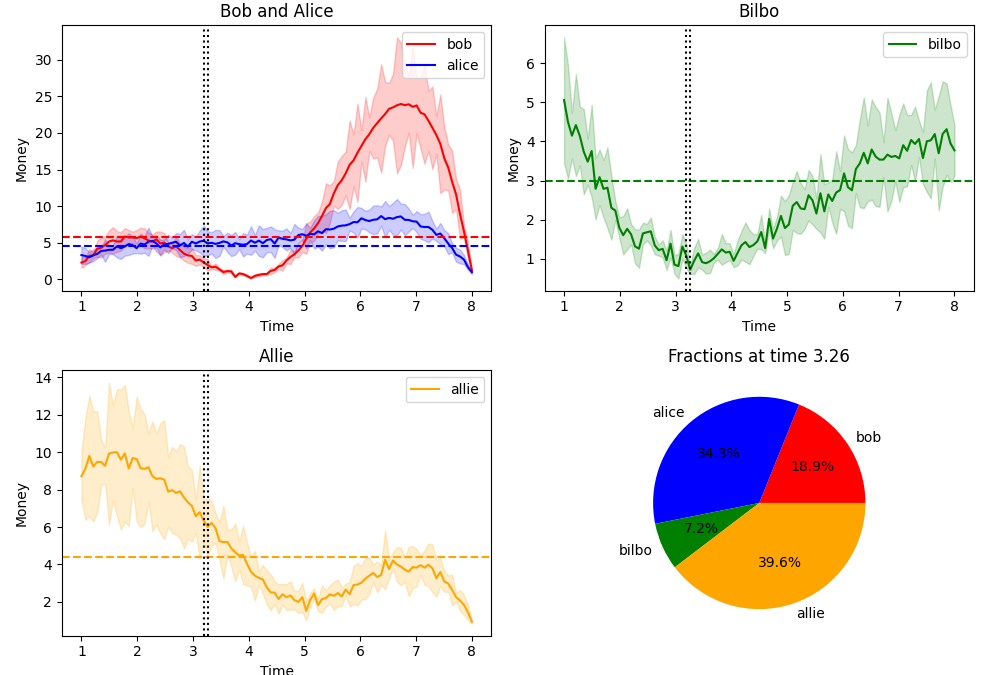
\includegraphics[width=0.49\textwidth]{figures/ff_1.png}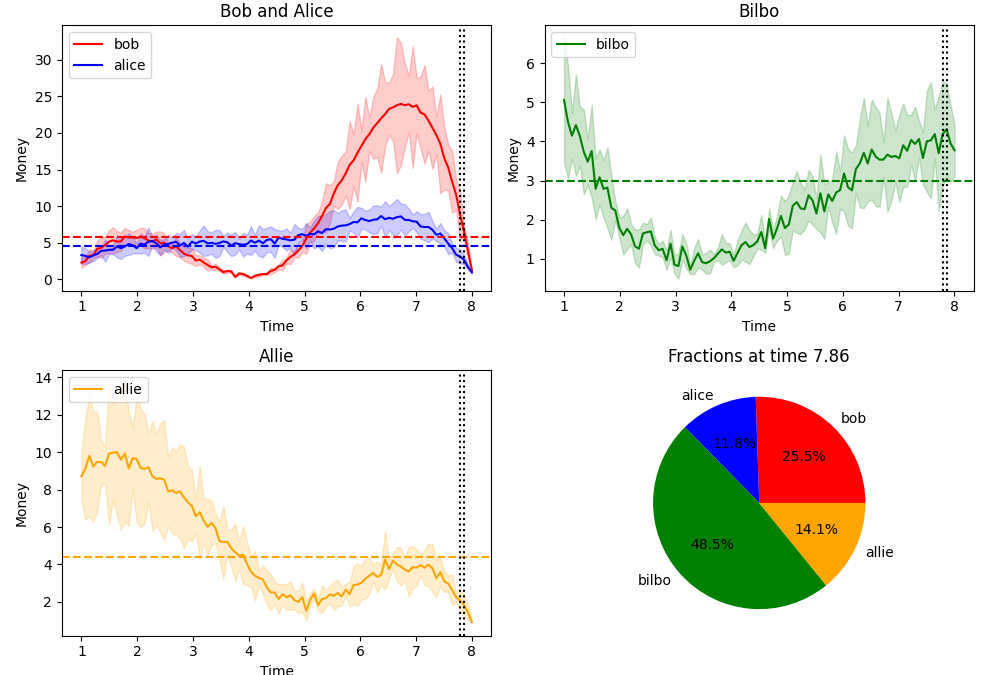
\includegraphics[width=0.49\textwidth]{figures/ff_2.png}
\end{AIbox}
%\caption{}
\end{figure}


We already see an example in Figure~\ref{fig:prelimexamples}. In the example, the plot produced by \DV\ appears to have a high density of data points, but in fact it only received 20 input values. \DV\ successfully created curves that oscillate smoothly, as instructed by the prompt. The error bar also varies randomly within the specified range of $10\% - 40 \%$, creating a realistic effect. We also challenged \DV\ by asking it to animate the pie chart, and gave it a really vague command ``animate the other three to match the pie chart''. \DV\ interprets the command perfectly. The plot shows \DV\'s exceptional ability to code and understand human instructions. Below we show another example demonstrating this ability in Figure~\ref{fig:plot-2}.
\\
\begin{figure}[H]
\begin{AIbox}{\DV}
{\bf Prompt:} \begin{minted}[breaklines, breaksymbol=, baselinestretch=1, fontsize=\scriptsize]{html}
Can you write a pyplot code of the following 3D plot:
Dot plot x(t), y(t), z(t) = (1 - t)^0.5 * sin(5* pi * t), (1 - t)^0.5 *cos(5* pi * t), C*(1 - t) + 0.5(1 - C * C).
-I want to have 101 dots in the interval, from t = 0 to t = 1 with a gap 0.01. Name the dote d_1, d_2, ..., d_{101} where d1 is for t = 0 and d_{101} is for t = 101
-I want to animate the plot using the following way:
-The colors of the dots form a rainbow, and it's changing gradually every 0.2 seconds.
-The size of the i-th dot is proportional to i^1.5.
-Initially, C = 1, and C changes from 1 to 0 and then from 0 to 1 every 10 seconds.
-Add a horizontal plane in the plot, the z-axis is the current mean of those points.
\end{minted}
\vspace{-0.3cm}
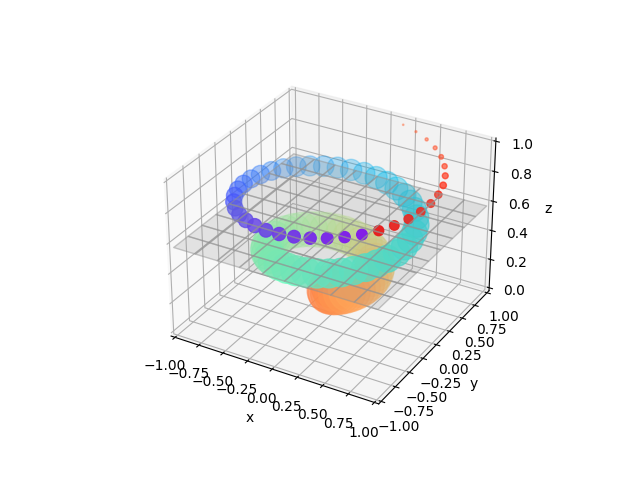
\includegraphics[trim={0 0 4cm 0}, width=0.4\linewidth]{figures/p4.png}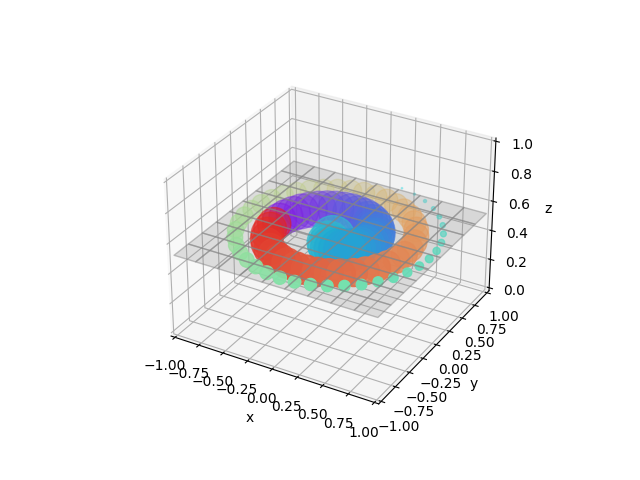
\includegraphics[trim={0 0 4cm 0}, width=0.4\linewidth]{figures/p3.png}
\end{AIbox}
\caption{The stunning visualization created by \DV \ from vague human instructions. \DV \ successfully interprets what it means by ``colors form a rainbow and changing gradually every 0.2 seconds'', \DV \ also sets all other details in the plot exactly as instructed, \emph{including the timings}.}
\label{fig:plot-2}
\end{figure}

% \subsubsection{Deep learning implementation}
% Arguably, one of the most important coding applications these days is deep learning. However, implementing a customized deep learning module from scratch can be a challenging task, as it requires not only familiarity with a specialized package such as Pytorch, but also a deep understanding of the underlying concepts and principles of deep learning models.

% \emph{We argue that \DV\ writes expert-level deep learning code, that is standardized and equipped with accurate comments for readability}, as we illustrate with an example of a novel and sophisticated optimizer in Pytorch that we design with \DV\.

% The \DV\ model shows impressive ability to infer the details of the optimizer logic and the Pytorch syntax from the prompt, and to generate code that is consistent and efficient. Remarkably, \DV\ understands what it means to `apply momentum' from the prompt. This is a non-trivial task that requires knowledge of the Pytorch syntax and the optimizer logic (i.e., momentum requires storing/reading the moving average into/from a separate state buffer). In comparison, ChatGPT does not know how to apply momentum at all, as it fails to realize the need for a state buffer and simply naively adds to the update the $W_k$ multiplied by the momentum coefficient (line labeled in red). This shows a difference between \DV\ and ChatGPT: While ChatGPT still relies on ``pattern matching'' to simply multiply momentum to the update, \DV\ understands what is momentum and translates the domain knowledge to accurate code. 
% \begin{figure}[H]
% \begin{AIbox}{\DV~vs ChatGPT}
% {\bf Prompt:} 
% \begin{minted}[breaklines, breaksymbol=, baselinestretch=1, fontsize=\tiny]{html}
% I want to write a customized optimizer in pytorch, the optimizer should do:
% 1. the parameters for the optimizer is learning rate, momentum ,weigth decay, d_dim, k and factor alpha
% 2. the optimizer goes through each parameter in the network, and then
% -- Get the gradient of this parameter, reshape it to 2D by looping through the dimensions, and keeping the dimension whose actual dimension (shape) is equal to d_dim, do an SVD decomposition of the parameter so W = U\Sigma V. 
% -- Keep the top k singular vectors of W, so we get a new matrix W_k = U \Sigma_k V. 
% -- Keep the top 2k singular vectors of W, so we get a new matrix W_{2k} = U \Sigma_{2k} V. 
% -- Normalize W_k according to the momentum of the F-norm of W_{2k}.
% -- Truncate each coordinate of W_k to the top alpha  percentile of all the coordinates, in absolute value.
% -- Apply momentum on W_k, and then update the network parameters using this momentum.
% -- Apply weight decay.
% \end{minted}

% {\bf \DV:}
% \begin{minted}[breaklines, breaksymbol=, baselinestretch=1, fontsize=\tiny]{python}
% import torch
% from torch.optim import Optimizer
% class CustomOptimizer(Optimizer):
%     ...

%     def step(self, closure=None):
%         ...
%                 # Perform SVD on the gradient matrix
%                 u, s, v = torch.svd(grad_2d)
%                 # Keep the top k singular vectors and values
%                 u_k = u[:, :k]
%                 s_k = s[:k]
%                 v_k = v[:, :k]
%                  # Keep the top 2k singular vectors and values
%                 u_2k = u[:, :2*k]
%                 s_2k = s[:2*k]
%                 v_2k = v[:, :2*k]
%                 # Reconstruct the gradient matrix with rank k
%                 grad_k = u_k @ torch.diag(s_k) @ v_k.t()
%                 # Normalize the gradient matrix with the momentum of the F-norm of the rank 2k matrix
%                 grad_2k_norm = torch.norm(s_2k)
%                 state = self.state[p]
%                 if 'grad_2k_norm_avg' not in state:
%                     # Initialize the moving average of the F-norm
%                     state['grad_2k_norm_avg'] = grad_2k_norm
%                 else:
%                     # Update the moving average of the F-norm
%                     state['grad_2k_norm_avg'] = momentum * state['grad_2k_norm_avg'] + (1 - momentum) * grad_2k_norm
%                 grad_k = grad_k / state['grad_2k_norm_avg']
%                 # Truncate each coordinate of the gradient matrix to the top alpha percentile of the absolute values
%                 grad_k_abs = grad_k.abs()
%                 threshold = grad_k_abs.kthvalue(int(alpha * grad_k_abs.numel()), dim=None).values
%                 grad_k = grad_k.clamp(min=-threshold, max=threshold)
%                 # Apply momentum on the gradient matrix
%                 if 'grad_k_momentum' not in state:
%                     # Initialize the momentum buffer
%                     state['grad_k_momentum'] = torch.zeros_like(grad_k)
%                 # Update the momentum buffer
%                 state['grad_k_momentum'] = momentum * state['grad_k_momentum'] - lr * grad_k
%                 # Update the parameter data with the momentum buffer
%                 param.add_(state['grad_k_momentum'])
%         ...
% \end{minted}

% {\bf ChatGPT:}
% \begin{minted}[breaklines, breaksymbol=, baselinestretch=1, fontsize=\tiny, highlightlines={16}, highlightcolor=pink]{python}
% import torch
% class CustomOptimizer(torch.optim.Optimizer):
%     ...
%     def step(self, closure=None):
%         ...
%             lr = group['lr']
%             momentum = group['momentum']
%             weight_decay = group['weight_decay']
%             ...
%                 grad = p.grad.data
%                 grad_2d = grad.view(-1, d_dim)
%                 U, S, V = torch.svd(grad_2d)
%                 W_k = U[:, :k] * S[:k] @ V[:k, :]
%                 W_k = W_k / torch.norm(W_k, p='fro')
%                 W_k = torch.where(torch.abs(W_k) > torch.topk(torch.abs(W_k), int(alpha * W_k.numel()))[0][-1], W_k, 0)
%                 p.data = p.data - lr * (momentum * W_k + weight_decay * p.data)
%     ...
% \end{minted}
% \end{AIbox}
% \caption{\DV~vs ChatGPT at implementing a customized Pytorch optimizer module. We label in red ChatGPT's mistake at `applying momentum'. }
% \end{figure}

%This is incorrect and does not reflect the intended optimizer logic. This shows that ChatGPT lacks the necessary domain knowledge and the ability to reason logically from the prompt.

%The code defines a class that inherits from torch.optim.Optimizer, and implements the required methods: init() and step(). In each step, it computes the spectrally truncated second moment of gradients, $W_k$, and its Frobenius norm, $W_{2k}$, for each parameter. It then normalizes $W_k$ by dividing it by the product of $W_{2k}$ and a momentum factor, which controls the degree of smoothing. It then updates the state buffer of the parameter with the moving average of $W_k$, using the momentum formula. Finally, it updates the parameter by subtracting the learning rate times the state buffer, and applying weight decay. The code is concise, readable, and follows the Pytorch conventions. Remarkably, \DV\ understands what it means to `apply momentum' from the prompt. This is a non-trivial task that requires knowledge of the Pytorch syntax and the optimizer logic (i.e., momentum requires storing/reading the moving average into/from a separate state buffer).
\vspace{-3mm}
\subsection{Coding interactive environments}
Programming for interactive environments entails various aspects of software development, such as choosing appropriate languages, tools, frameworks, and paradigms based on the project's objectives and constraints. The main challenge in this domain is to use event-driven programming to handle user input, timer, and other asynchronous events, design user interfaces that are intuitive and coherent, and implement game loops that manage the state and logic of the environment. We show that \DV\ can produce code that can tackle these challenges effectively. 


%\subsubsection{Game development}
%Game development is a complex and creative process that requires a large amount of domain knowledge from different fields. A typical game development pipeline may consist of the following stages:
%\begin{itemize}
%    \item\textbf{Game Play:} This is the core of the game, where the designer creates the rules, mechanics, goals, challenges, and rewards that define how the player interacts with the game and what experience they have. To design engaging and satisfying gameplay, the designer needs to have domain knowledge of game design principles, genres, conventions, user interface, feedback, balance, difficulty, and fun. The designer also needs to consider the target audience, the platform, the genre, and the market of the game.
 %   \item\textbf{Art:} This is the stage where the artist creates the visual elements, such as graphics, animations, models, textures, lighting, and effects, that convey the game's aesthetic, style, and mood. To create appealing and expressive art, the artist needs to have domain knowledge of art principles, tools, techniques, genres, and trends. The artist also needs to collaborate with the designer and the programmer to ensure the art matches the gameplay and the technical requirements of the game.
  %  \item\textbf{Programming}: This is the stage where the programmer creates the code, algorithms, data structures, and systems that implement the game's functionality, logic, and performance. To create robust and efficient code, the programmer needs to have domain knowledge of programming languages, paradigms, frameworks, libraries, platforms, and optimization. The programmer also needs to collaborate with the designer and the artist to ensure the code supports the gameplay and the art of the game. 
%\end{itemize}

%Depending on the scope, scale, and complexity of the game, a game designer may need to have some or all of these domain knowledge areas, or work with a team of specialists who have them. Additionally, a game designer may also need to have domain knowledge of the specific topic, theme, or genre of the game, such as history, science, fantasy, horror, etc., to ensure accuracy, authenticity, and creativity.

%However, with the help of \DV\, the art and programming stages can be left to the \DV\ system, which can generate high-quality and customized art and code for any game concept. This allows the human designers to focus fully on the gameplay aspect, and explore their vision and ideas without the limitations and challenges of the traditional pipeline. \DV\ can also provide feedback, suggestions, and inspiration to the human designer, creating a collaborative and dynamic game development process.

%raster columns=2, raster rows=2,size=small,
%%\begin{tcbraster}[  raster equal height, raster halign=center, raster valign=center]
\begin{figure}[H]
\begin{AIbox}{\DV}
{\bf\scriptsize Prompt:} \vspace{-5px}
\begin{minted}[breaklines, breaksymbol=, baselinestretch=1, fontsize=\scriptsize]{html}
Can you write a 3D game in HTML with Javascript, I want:
-There are three avatars, each is a sphere.
-The player controls the avatar using arrow keys to move.
-The enemy avatar is trying to catch the player.
-The defender avatar is trying to block the enemy.
-There are also random obstacles as cubes spawned randomly at the beginning and moving randomly. The avatars can not cross those cubes.
-The player moves on a 2D plane surrounded by walls that he can not cross. The wall should cover the boundary of the entire plane. 
-Add physics to the environment using cannon.
-If the enemy catches the player, the game is over.
\end{minted}
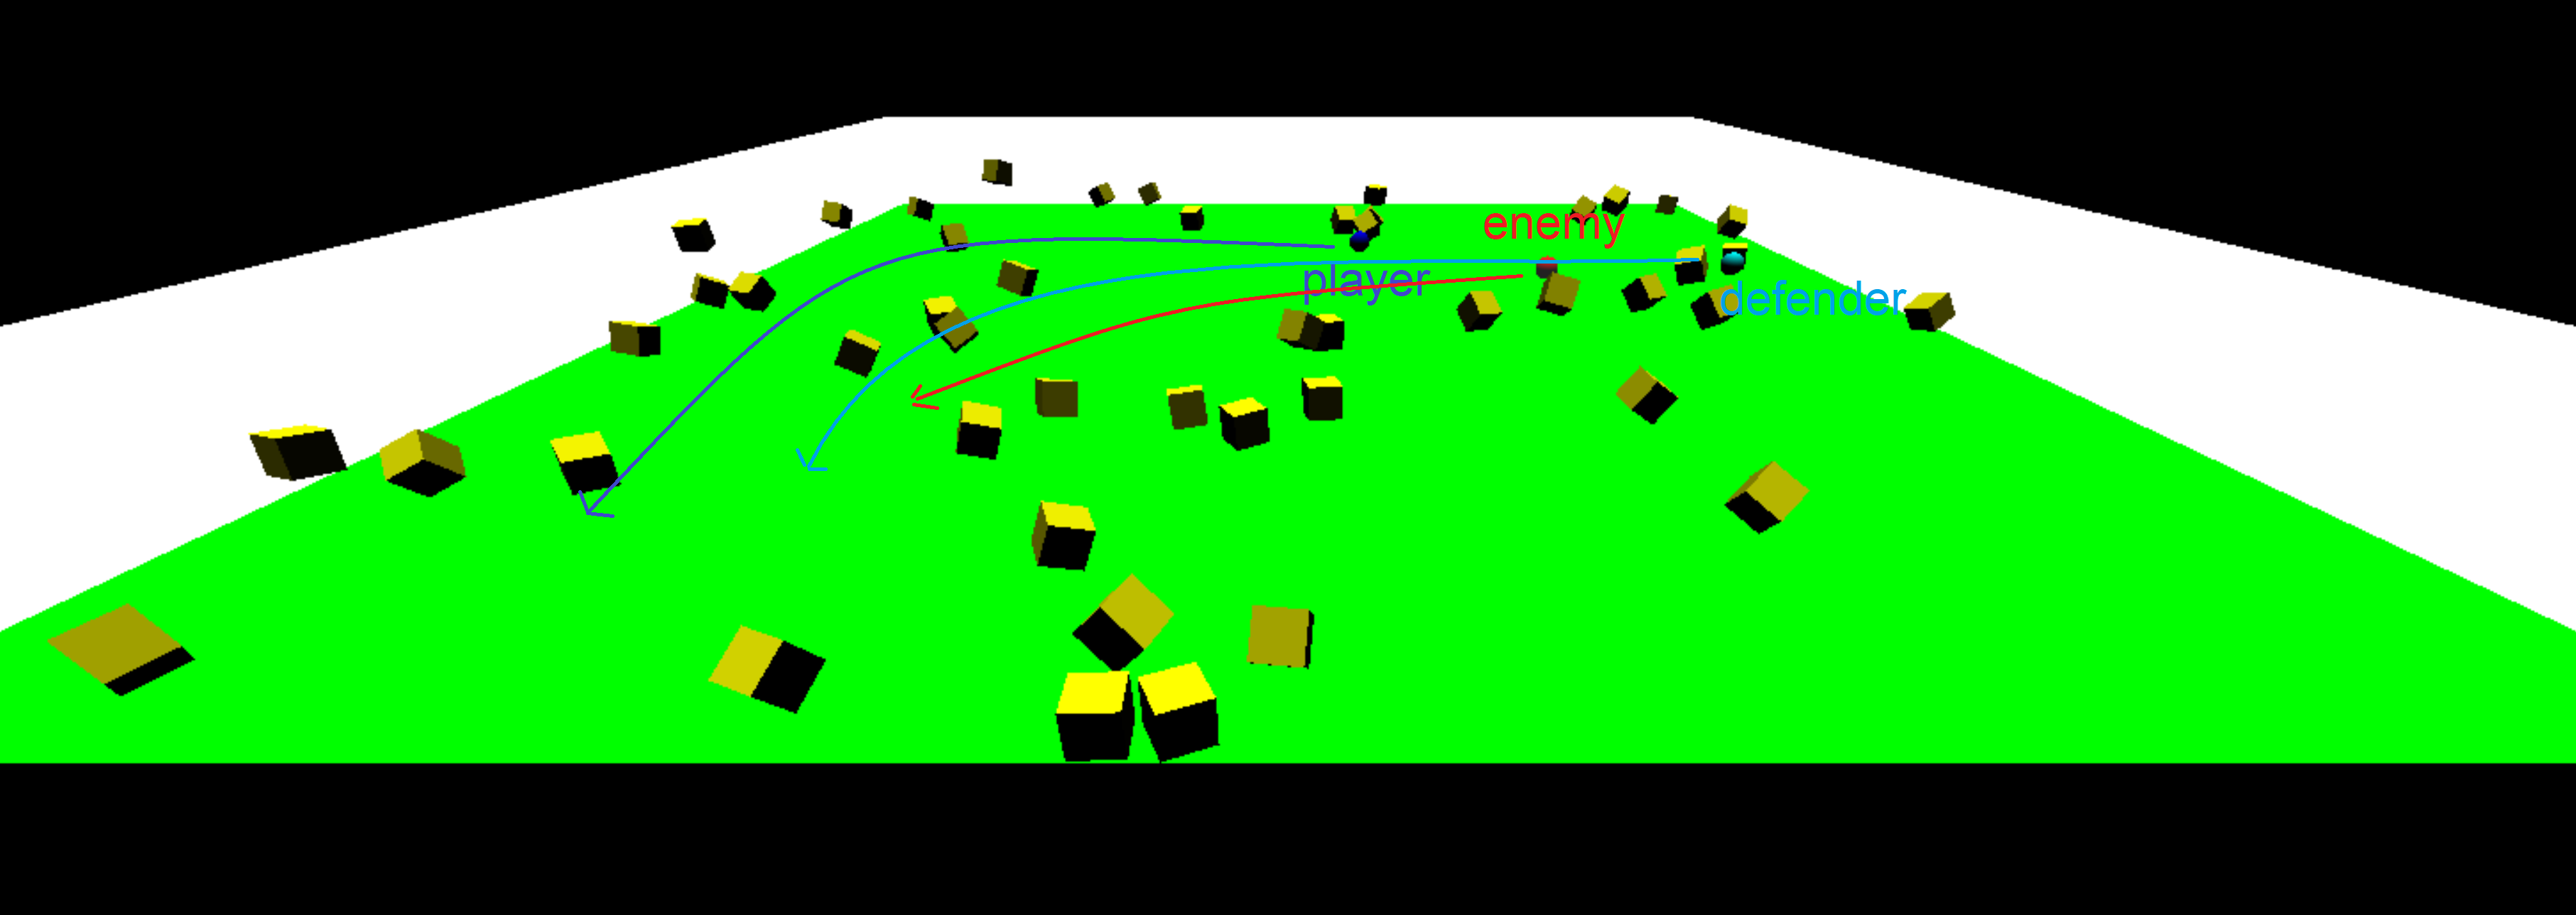
\includegraphics[height=0.17\linewidth]{figures/g1.png} \hfill
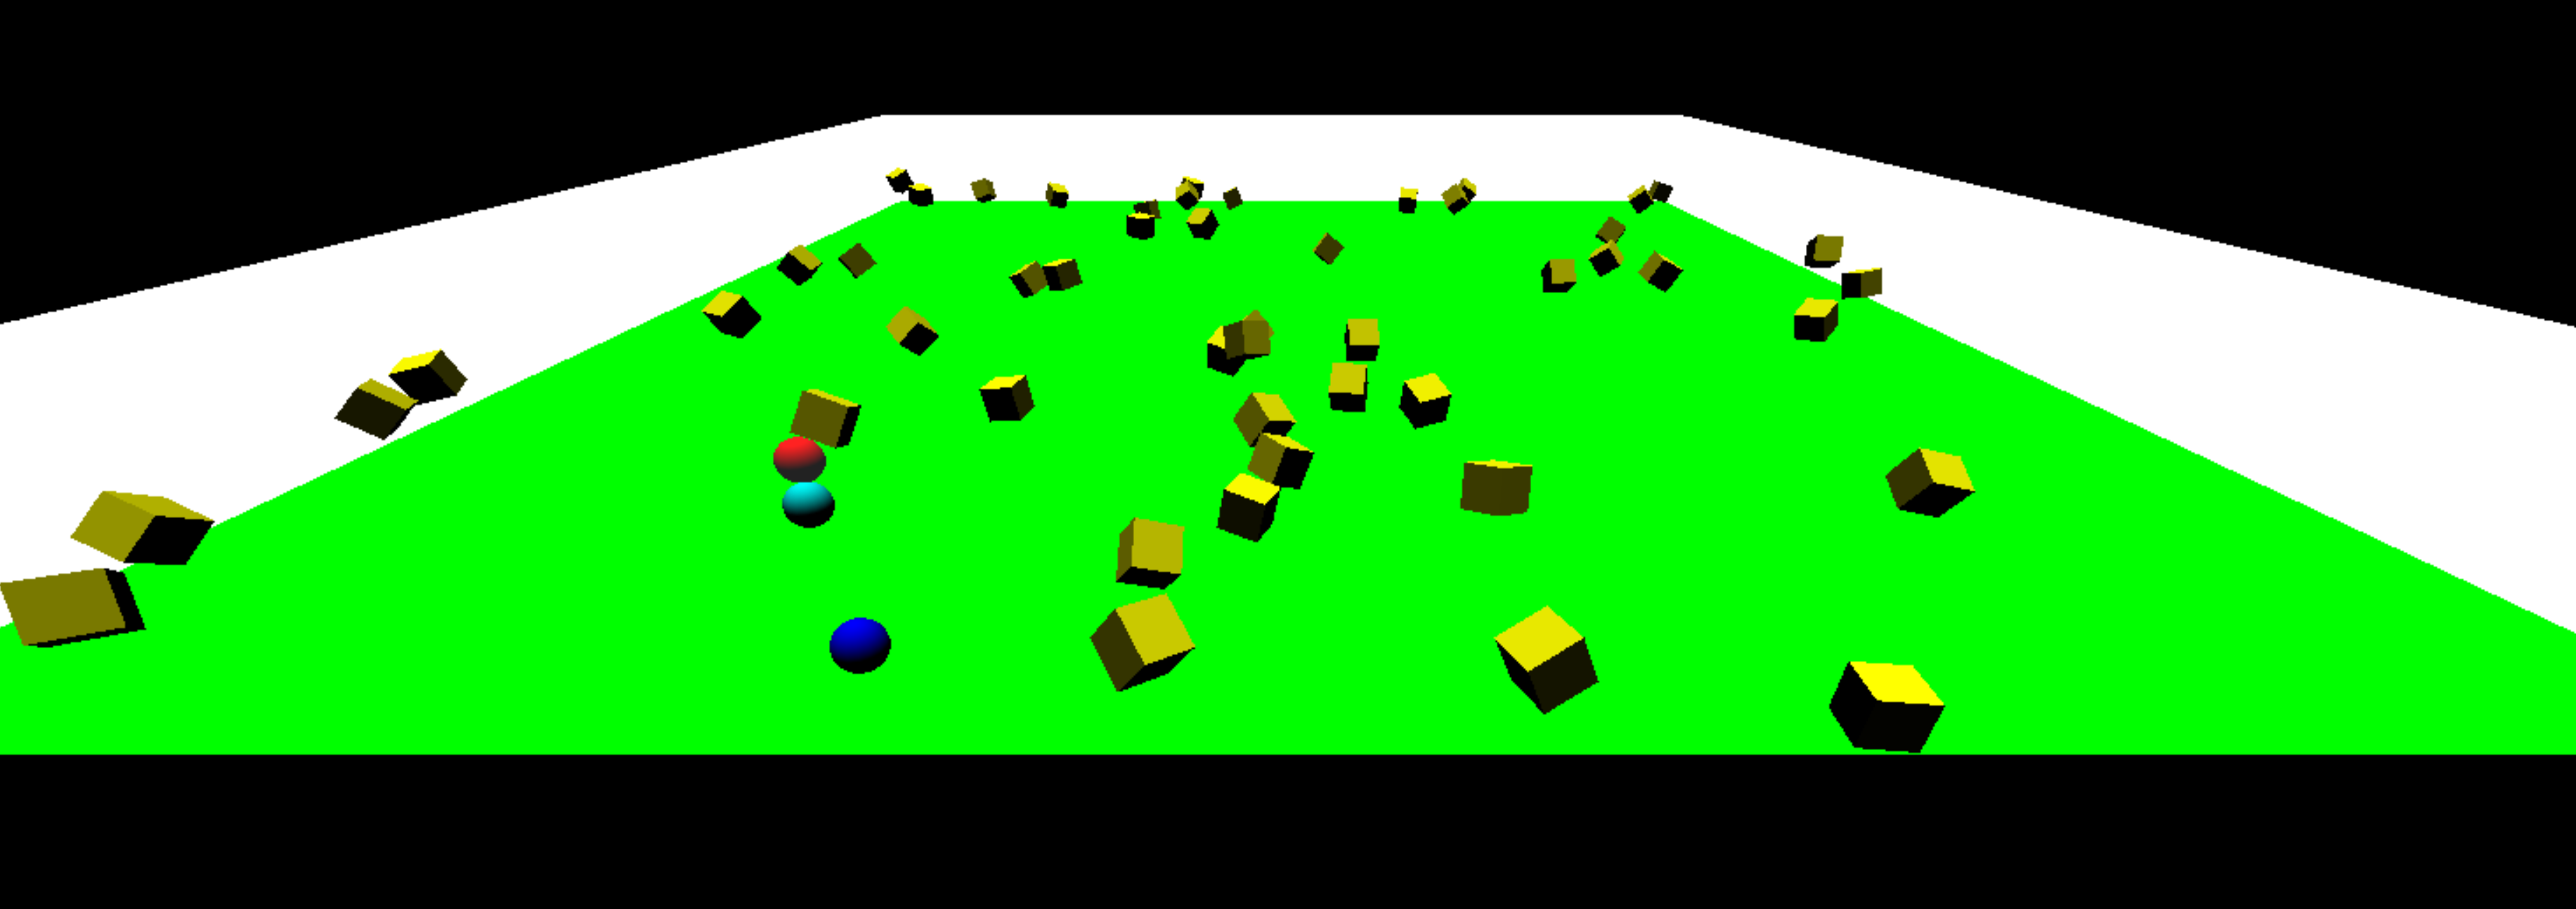
\includegraphics[height=0.17\linewidth]{figures/g2.png}
\end{AIbox}
\caption{\DV develops 3D games. The arrow illustrates the expected behaviors of the player, enemy and defender in the game.}
\end{figure}
\begin{figure}[H]
\begin{AIbox}{\DV}
{\bf\scriptsize Prompt:} \vspace{-5px}
\begin{minted}[breaklines, breaksymbol=, baselinestretch=1, fontsize=\scriptsize]{html}
Can you write a 2D tank war game in HTML with Javascript? You can use a square to represent the tank, a triangle to represent the front of the tank, and use a ball to represent the bullet shell. I want to generate some random walls at the beginning of the game, and when the shell hits the wall, the wall disappears. The player wins the game if he destroys all enemy tanks. If the player's tank gets hit, then he loses the game. The player uses WASD to control the moves of the tank, and uses space to fire a shell. The enemy tanks are moving randomly and fire randomly.
\end{minted}
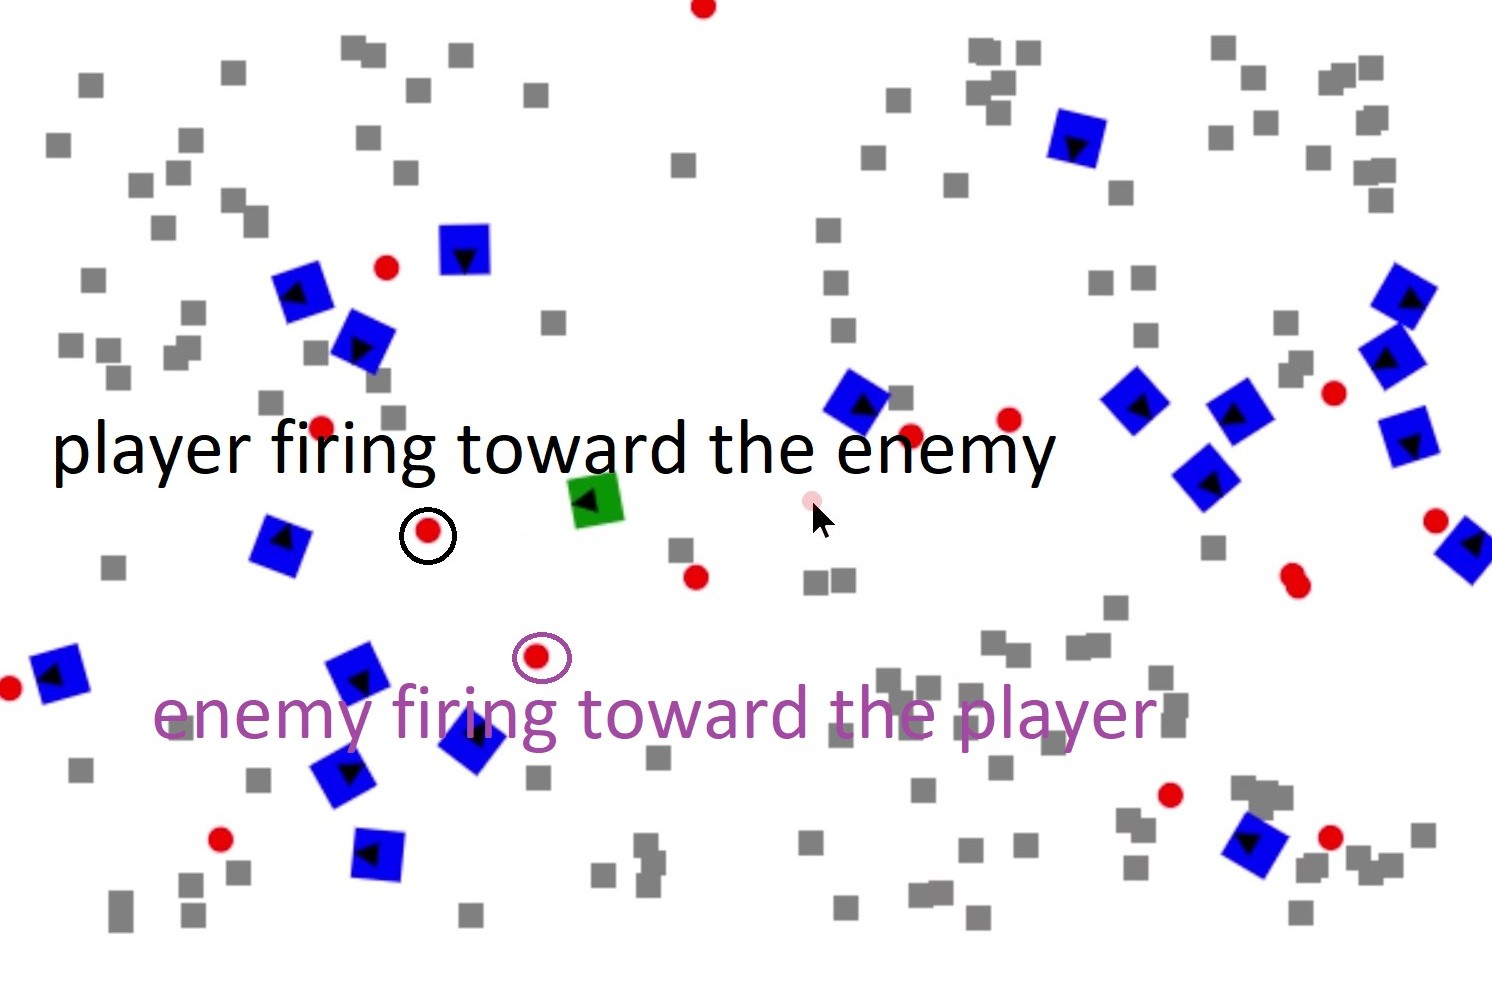
\includegraphics[height=0.25\linewidth]{figures/t011.jpg} \hfill 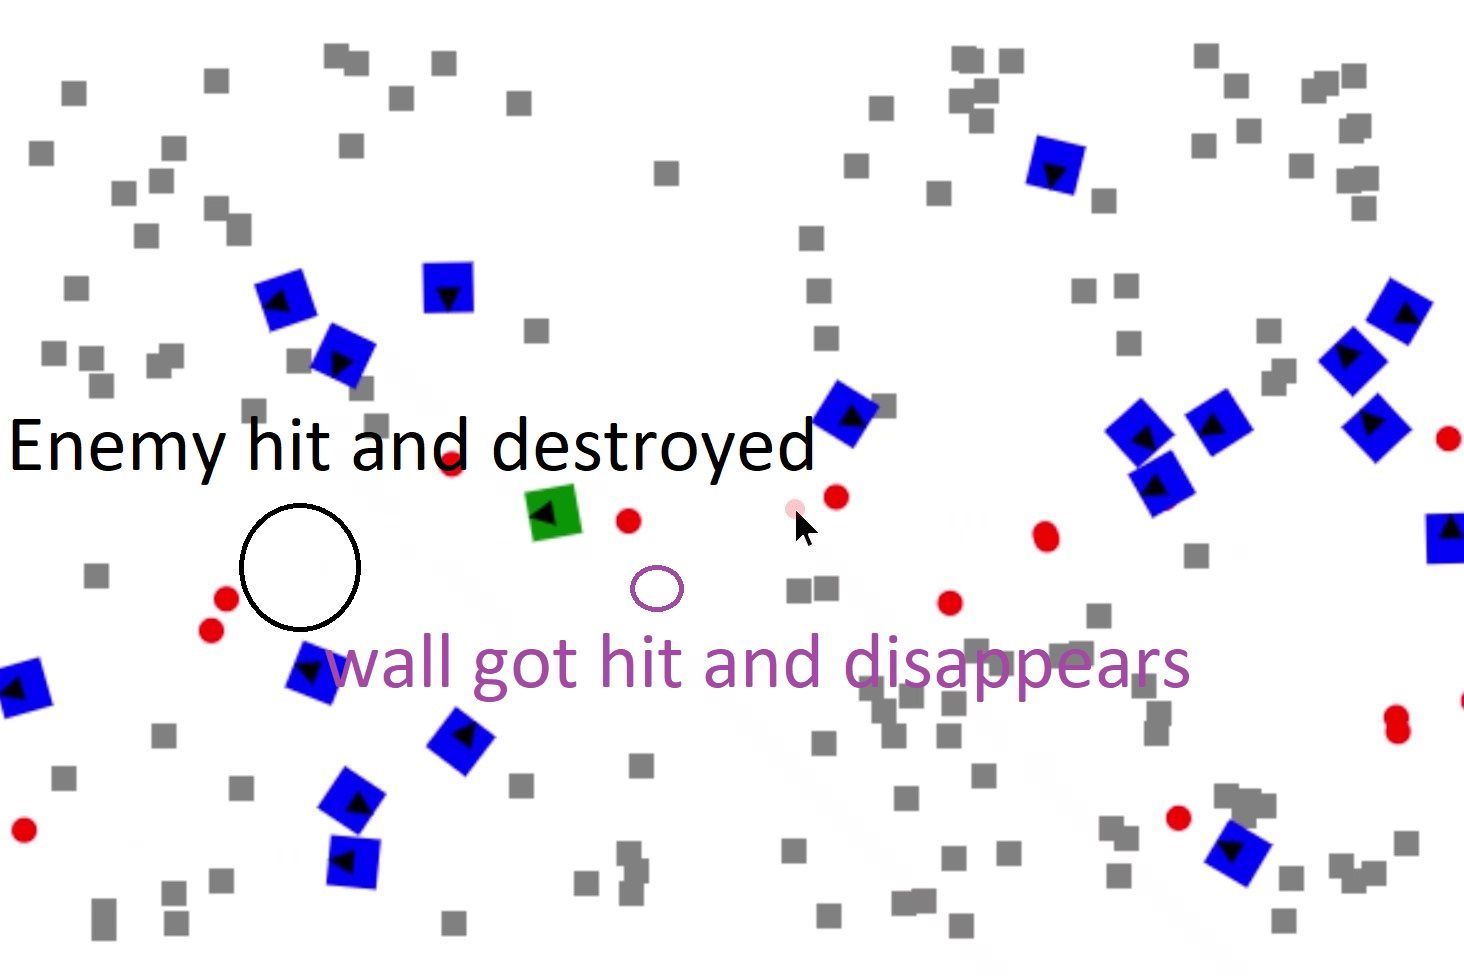
\includegraphics[height=0.25\linewidth]{figures/t02.jpg}
\end{AIbox}
\caption{\DV~ develops complex 2D games. }
\end{figure}
To illustrate the capabilities of \DV\ in the zero-shot game generation, we show two examples of games that involve interpreting human intent, managing game states, and handling various types of timers and events. These games are complex and require a comprehensive understanding from \DV\. \DV\ accurately generates the code that matches the specifications: The player's movement is controlled accurately using arrow keys. The obstacles are cubes that move randomly, the white walls and the obstacles prevent the player/enemy/defender from passing through, and the enemy (red ball) follows the player. Moreover, \DV\ correctly interprets the meaning of "block" and implements the logic for the defender to position itself between the player and the enemy.  This example showcases the remarkable ability of \DV\ to translate natural language instructions into code.



Arguably, such 3D HTML game can take an expert a couple hours to complete, while \DV\ generates the entire $\ge 500$ lines of code in less than one minute. Again, the potential impact of \DV\ on (simple) game development can be transformative.

The 2D game involves complex logic and state management for the enemy, player, shell, and wall objects. The program also needs to handle object interactions, such as collisions, to prevent the player and enemies from passing through the walls, and to detect when a bullet hits a target or a wall. \DV\ accurately captures all the details, including the square and triangular shapes of the tanks, the different colors for the player and enemy, and the contrast between the tank and the triangle colors. \DV~correctly codes the state variables and transitions for all the objects and infers from common sense that a shell should disappear when it hits a wall and implements that feature. The program, which consists of $\approx 600$ lines of code, is generated by \DV\ in about a minute and runs without any errors.

We also give more examples of \DV's strong GUI programming ability in Section~\ref{sec:code_appendix}. 
%Here we present two examples of how to use \DV\ as a game engine that can generate games in 2D and 3D, based on high-level specifications of game plays from prompts, such as the genre, the setting, the goals, the mechanics, and the challenges. \DV\ allows users to quickly prototype and test their game ideas, without requiring any programming or art skills.

%Furthermore, since we did not specificy a name for either of the games, we present the written javascript snippets back to \DV\ and ask it to ``come up with suggestions for creative, catchy, and descriptive names for the games". \DV\'s suggestions are as follows
%\begin{itemize}
%    \item for the 3D game: \emph{Escape the Red ball, Bounce and Dodge, Sphere Chase, Ballistic, Flee the Field}
 %   \item for the 2D game: \emph{Tank Blast, Wall Breaker, Shell Shock, Tank Trouble}
%\end{itemize}




\subsection{\DV\ grasps profound programming knowledge}

\DV\ grasps profound programming knowledge that are essential for developing efficient and secure software systems. Unlike other models that may only handle high-level languages or frameworks, \DV\ can dive into the low-level details of how the code interacts with the hardware and the operating system.

\paragraph{Example I: memory alignment in C/C\texttt{++}.} \DV\ understands the struct memory alignment rule in the C programming language, which determines how the compiler organizes the fields of a structure in the memory. This rule affects the size, performance, and portability of the code, and may also introduce security vulnerabilities if not handled properly. In this example, we define two semantically identical struct objects in C but with variables declared in different orders. According to the memory alignment rule, the ordering makes a difference in the memory consumption of the structs. For instance, for the objects \textbf{mystruct\textunderscore A} and \textbf{mystruct\textunderscore B} defined in the prompt of Figure~\ref{fig:code-memory-align}, they consist of exactly the same member variables: 1 \textbf{int} type and 2 \textbf{char} type. However, they occupy different sizes in memory due to declaration order of the variables.


We test whether \DV\ can tell the sizes in bytes of the struct objects. \DV\ not only outputs the correct numbers for the size of the structs, it also provides a convincing explanation. This capability signifies \DV\'s deep understanding of how the C programming language interacts with operating systems under the hood. On the contrary, we see ChatGPT is not aware of the memory alignment rule or its implications. 

\begin{figure}[H]
\begin{AIbox}{\DV~vs ChatGPT}
{\bf Prompt} 
\begin{minted}[breaklines, breaksymbol=, baselinestretch=1, fontsize=\tiny]{cpp}
    struct mystruct_A {  char a; int b; char c; } x;
    struct mystruct_B {  int b;  char a; char c; } y;
    
    #include <stdio.h>
    int main(void) {
        printf("Size of x: %zu bytes\n", sizeof(x)); 
        printf("Size of y: %zu bytes\n", sizeof(y));
        return 0;
    }
    
    Possible Output:
\end{minted}


\parbox[t]{0.53\linewidth}{{\bf \DV:} 
\tiny
\begin{alltt}
There are different ways to implement and align structures in memory, so the exact output may vary depending on the compiler, platform, and options used. However, one possible output is:\\

Size of x: 12 bytes\\
Size of y: 8 bytes\\

This output assumes that the compiler uses 4-byte alignment for structures, meaning that each structure member starts at an offset that is a multiple of 4 bytes from the beginning of the structure. This may result in some padding bytes being inserted between or after the members to maintain alignment. For example, in x, there may be 3 padding bytes after a and 3 padding bytes after c, while in y, there may be no padding at all. The size of a structure is the sum of the sizes of its members plus any padding bytes.
\end{alltt}
}\hspace{0.02\linewidth}%
\parbox[t]{0.45\linewidth}{{\bf ChatGPT:}
\tiny
\begin{alltt}
Size of x: 8 bytes\\
Size of y: 8 bytes\\

The output of this code would be the size of the two structures in bytes. The size of a structure in C is the sum of the sizes of all of its members. In this case, the size of mystruct\textunderscore A is the size of a char plus the size of an int plus the size of another char, which is \fcolorbox{aired}{aired}{1 + 4 + 1 = 8} bytes. \\
\\
Similarly, the size of mystruct\textunderscore B is also 8 bytes. This means that both structures will be allocated the same amount of memory. \\
\\
\fcolorbox{aired}{aired}{Note that the order in which the members are}
\fcolorbox{aired}{aired}{declared in the structure does not affect its}
\fcolorbox{aired}{aired}{size.}
\end{alltt}
}
\end{AIbox}
\caption{\DV vs ChatGPT on the~memory alignment rule of C/C\texttt{++}. Mistakes are labeled in red.}
\label{fig:code-memory-align}
\end{figure}



\paragraph{Example II: Reverse engineering} \DV\ also has a surprising ability for reverse engineering. Reverse engineering is an essential test for software security which amounts to search for useful information in a executable program written in a machine-readable (i.e., binary) representation of CPU instructions. It is a challenging task that requires understanding the syntax, semantics, and conventions of assembly language, as well as the architecture and behavior of the processor and the operating system. \DV\ exhibits proficiency in analysis tools such as ltrace, lldm, Hopper and can reverse engineer assembly code and generate the original C code that produced it. In this example, our goal is to crack a binary executable file that requires a password to run. To achieve this, we communicate with \DV\, a virtual assistant that can suggest tools and techniques for binary analysis. \DV\ guides us through different steps and we follow them, running commands and tools on our computer and reporting the results to \DV\. \DV\ shows us how to use various methods, such as:
\begin{itemize}
    \item Checking the file format and metadata with tools like file and strings
    \item Disassembling the code with tools like objdump and radare2
    \item Debugging the code with tools like gdb and ltrace
    \item Applying reverse engineering techniques like patching, hooking, and decompiling
\end{itemize}
During this process, \DV\ discovers a clue in the assembly code of the file: the password is compared to a hash value that is derived from a simple mathematical formula. Based on this clue, \DV\ writes a python program that tries different combinations of numbers until it finds the one that matches the hash value. This program reveals the password that we need to run the file and crack it. \DV\ demonstrates its ability to use diverse and effective methods for binary analysis and cracking. In Appendix~\ref{appendix:reverse-engine}, we present an abbreviated log of the conversation.

In fact, \DV exhibits all-around proficiency in utilizing existing tools also beyond programming, which we will discuss in details in Section~\ref{sec:affordances}.



\subsection{\DV\ can execute code}

We have shown that \DV \ can generate high-quality code, but does it also comprehend the functionality of the code it produces? In this section, we evaluate \DV's capacity to execute the code, demonstrating that \DV \ also understands and can effectively track the intricate execution states of the code.

We begin with the following dynamic programming example: 
\begin{figure}[H]
\begin{AIbox}{\DV}
{\bf Prompt:}\\
{\tiny
I have the following python code:
\vspace{-0.3cm}
\begin{minted}[breaklines, breaksymbol=, baselinestretch=1, fontsize=\tiny]{python}
def to_str(i, j):
    return str(i) + "," + str(j)
dict = {}
def DP(i, j):
    if i <= 0 or j <= 0:
        dict[to_str(i, j)] = abs(4 * j - 3 * i) 
    elif to_str(i, j) not in dict.keys():
        arr = []
        for ir in range(i):
            for jr in range(j):
                arr.append(DP(ir, jr))
        dict[to_str(i, j)] = max(arr)
    return dict[to_str(i, j)]
\end{minted}
\vspace{-0.3cm}
What is the result of DP(3, 4)? Write down the execution with intermediate steps.
}\\
{\bf\DV:}
\begin{minted}[breaklines, breaksymbol=,  fontsize=\tiny]{html}
DP(3, 4):
- i > 0 and j > 0, so we don't return from the first if statement
- to_str(3, 4) is not in dict, so we enter the second if statement
- arr = []
- We loop through ir from 0 to 2, and jr from 0 to 3
  - to_str(0, 0)  is not in dict, so DP(0, 0) returns abs(4 * 0 - 3 * 0) = 0, dict =  {"0,0": 0}, arr = [0]
  - to_str(0, 1)  is not in dict, so DP(0, 1) returns abs(4 * 1 - 3 * 0) = 4, dict =  {"0,0": 0, "0,1": 4}, arr = [0, 4]
  - to_str(0, 2)  is not in dict, so DP(0, 2) returns abs(4 * 2 - 3 * 0) = 8, dict =  {"0,0": 0, "0,1": 4, "0,2": 8}, arr = [0, 4, 8]
  - to_str(0, 3)  is not in dict, so DP(0, 3) returns abs(4 * 3 - 3 * 0) = 12, dict =  {"0,0": 0, "0,1": 4, "0,2": 8, "0,3": 12}, arr = [0, 4, 8, 12]
  - to_str(1, 0)  is not in dict, so DP(1, 0) returns abs(4 * 0 - 3 * 1) = 3, dict =  {"0,0": 0, "0,1": 4, "0,2": 8, "0,3": 12, "1,0": 3}, arr = [0, 4, 8, 12, 3]
  - to_str(1, 1)  is not in dict, so DP(1, 1) enters  the second if statement, arr1 = [] 
 - We loop through  ir from 0 to 0, and jr from 0 to 0
   - to_str(0, 0) is in dict, so DP(0, 0) returns 0, arr1 = [0]
 - dict["1,1"] = max(arr1) = 0, dict =  {"0,0": 0, "0,1": 4, "0,2": 8, "0,3": 12, "1,0": 3, "1,1": 0}, arr = [0, 4, 8, 12, 3, 0]
 - Continuing with the outer loop, to_str(1, 2) is not in dict, so DP(1, 2) enters the second if statement, arr2 = []
 - We loop through ir from 0 to 0, and jr from 0 to 1
   - to_str(0, 0) is in dict, so DP(0, 0) returns 0, arr2 = [0]
   - to_str(0, 1) is in dict, so DP(0, 1) returns 4, arr2 = [0, 4]
 - dict["1,2"] = max(arr2) = 4, dict =  {"0,0": 0, "0,1": 4, "0,2": 8, "0,3": 12, "1,0": 3, "1,1": 0, "1,2": 4}, arr = [0, 4, 8, 12, 3, 0, 4]
 - Continuing with the outer loop, to_str(1, 3) is not in dict, so DP(1, 3) enters the second if statement, arr3 = []
 - We loop through ir from 0 to 0, and jr from 0 to 2
   - to_str(0, 0) is in dict, so DP(0, 0) returns 0, arr3 = [0]
   - to_str(0, 1) is in dict, so DP(0, 1) returns 4, arr3 = [0, 4]
   - to_str(0, 2) is in dict, so DP(0, 2) returns 8, arr3 = [0, 4, 8]
 - dict["1,3"] = max(arr3) = 8, dict =  {"0,0": 0, "0,1": 4, "0,2": 8, "0,3": 12, "1,0": 3, "1,1": 0, "1,2": 4, "1,3": 8}, arr = [0, 4, 8, 12, 3, 0, 4, 8]
 - Continuing with the outer loop, to_str(2, 0) is not in dict, so DP(2, 0) returns abs(4 * 0 - 3 * 2) = 6, dict =  {"0,0": 0, "0,1": 4, "0,2": 8, "0,3": 12, "1,0": 3, "1,1": 0, "1,2": 4, "1,3": 8, "2,0": 6}, arr = [0, 4, 8, 12, 3, 0, 4, 8, 6]
 - Continuing with the outer loop, to_str(2, 1) is not in dict, so DP(2, 1) enters the second if statement, arr4 = []
 - We loop through ir from 0 to 1, and jr from 0 to 0
   - to_str(0, 0) is in dict, so DP(0, 0) returns 0, arr4 = [0]
   - to_str(1, 0) is in dict, so DP(1, 0) returns 3, arr4 = [0, 3]
 - dict["2,1"] = max(arr4) = 3, dict =  {"0,0": 0, "0,1": 4, "0,2": 8, "0,3": 12, "1,0": 3, "1,1": 0, "1,2": 4, "1,3": 8, "2,0": 6, "2,1": 3}, arr = [0, 4, 8, 12, 3, 0, 4, 8, 6, 3]
 - Continuing with the outer loop, to_str(2, 2) is not in dict, so DP(2, 2) enters the second if statement, arr5 = []
 - We loop through ir from 0 to 1, and jr from 0 to 1
   - to_str(0, 0) is in dict, so DP(0, 0) returns 0, arr5 = [0]
   - to_str(0, 1) is in dict, so DP(0, 1) returns 4, arr5 = [0, 4]
   - to_str(1, 0) is in dict, so DP(1, 0) returns 3, arr5 = [0, 4, 3]
   - to_str(1, 1) is in dict, so DP(1, 1) returns 0, arr5 = [0, 4, 3, 0]
 - dict["2,2"] = max(arr5) = 4, dict =  {"0,0": 0, "0,1": 4, "0,2": 8, "0,3": 12, "1,0": 3, "1,1": 0, "1,2": 4, "1,3": 8, "2,0": 6, "2,1": 3, "2,2": 4}, arr = [0, 4, 8, 12, 3, 0, 4, 8, 6, 3, 4]
 - Continuing with the outer loop, to_str(2, 3) is not in dict, so DP(2, 3) enters the second if statement, arr6 = []
 - We loop through ir from 0 to 1, and jr from 0 to 2
   - to_str(0, 0) is in dict, so DP(0, 0) returns 0, arr6 = [0]
   - to_str(0, 1) is in dict, so DP(0, 1) returns 4, arr6 = [0, 4]
   - to_str(0, 2) is in dict, so DP(0, 2) returns 8, arr6 = [0, 4, 8]
   - to_str(1, 0) is in dict, so DP(1, 0) returns 3, arr6 = [0, 4, 8, 3]
   - to_str(1, 1) is in dict, so DP(1, 1) returns 0, arr6 = [0, 4, 8, 3, 0]
   - to_str(1, 2) is in dict, so DP(1, 2) returns 4, arr6 = [0, 4, 8, 3, 0, 4]
 - dict["2,3"] = max(arr6) = 8, dict =  {"0,0": 0, "0,1": 4, "0,2": 8, "0,3": 12, "1,0": 3, "1,1": 0, "1,2": 4, "1,3": 8, "2,0": 6, "2,1": 3, "2,2": 4, "2,3": 8}, arr = [0, 4, 8, 12, 3, 0, 4, 8, 6, 3, 4, 8]
- dict["3,4"] = max(arr) = 12
- DP(3, 4) returns 12
\end{minted}
\end{AIbox}
\caption{\DV~executes Python code.}
\end{figure}

We can see that \DV \ accurately tracks the state of the code, including the loop, recursive calls, dictionary states, etc. This demonstrates that \DV \ not only knows how to write the code but also knows how it is implemented. In the following section, we show that \DV \ can leverage its knowledge to comprehend pseudo code -- This is even beyond the ability of any current compilers. 

\subsubsection{\DV\ can also execute pseudo code}

%\DV \ is capable of inferring the execution of standard code, however, one might still argue that this is ``pattern matching'', since the execution logs of the codes are sometimes available online. 

Today, compilers and platforms can execute code quickly and accurately, but they demand strict adherence to syntax and semantics. Compilers cannot handle vague or informal expressions, or natural language descriptions of functionality. In this section, we show how \DV\ can overcome these limitations and execute pseudo-code---code that is not written in a fixed format, or that contains natural language explanations of what the code should do. \DV\ can use its natural language understanding skills to interpret and execute pseudo-code.
%\textbf{comment that this only works if it outputs each intermediate step? }

\begin{figure}[H]
\begin{AIbox}{\DV}
{\bf Prompt:} \begin{minted}[breaklines, breaksymbol=, baselinestretch=1, fontsize=\scriptsize]{html}
I have a python function  merge_array, the function takes two arrays of length m, n respectively, and output a new array by merging the first m-1 element of the first array and the last n - 1 elements of the second array.
Suppose I call the merge_array function in the following way:
function rec
input: one array A, integer k
code: 
if the length of A is less than k, we first call rec(A + [length(A)], k) to get B
after that, call merge_array(B, B) to get C
return C.
if the length of A is larger or equal to k, return A.
end rec
Can you tell me what is the execution of rec([5, 10, 88], 6) with intermediate steps?
\end{minted}


{\bf \DV:}
\begin{minted}[breaklines, breaksymbol=, baselinestretch=1, fontsize=\scriptsize]{html}
One possible execution of rec([5, 10, 88], 6) with intermediate steps is:
- Since the length of A is 3, which is less than k = 6, we first call rec(A + [length(A)], k) to get B. That is, we call rec([5, 10, 88, 3], 6).
- In the recursive call, the length of A is 4, which is still less than k = 6, so we again call rec(A + [length(A)], k) to get B. That is, we call rec([5, 10, 88, 3, 4], 6).
- In the second recursive call, the length of A is 5, which is still less than k = 6, so we again call rec(A + [length(A)], k) to get B. That is, we call rec([5, 10, 88, 3, 4, 5], 6).
- In the third recursive call, the length of A is 6, which is equal to k = 6, so we return A as B. That is, we return [5, 10, 88, 3, 4, 5] as B.
- In the second recursive call, we have B = [5, 10, 88, 3, 4, 5], so we call merge_array(B, B) to get C. The merge_array function takes the first m - 1 = 5 elements of the first array and the last n - 1 = 5 elements of the second array and merges them into a new array. That is, C = [5, 10, 88, 3, 4, 10, 88, 3, 4, 5]. We return C as B.
- In the first recursive call, we have B = [5, 10, 88, 3, 4, 10, 88, 3, 4, 5], so we call merge_array(B, B) to get C. The merge_array function takes the first m - 1 = 9 elements of the first array and the last n - 1 = 9 elements of the second array and merges them into a new array. That is, C = [5, 10, 88, 3, 4, 10, 88, 3, 4, 10, 88, 3, 4, 10, 88, 3, 4, 5]. We return C as B.
- In the original call, we have B = [5, 10, 88, 3, 4, 10, 88, 3, 4, 10, 88, 3, 4, 10, 88, 3, 4, 5], so we return B as the final output of rec([5, 10, 88], 6).
\end{minted}
\end{AIbox}
\caption{\DV\ pseudo code execution}
\label{fig:pseudocode1}
\end{figure}


In the example above, \DV\ correctly interprets the informal description of the \textbf{merge\_array} function, which merges two arrays into one array with missing elements. It also understands the recursive function \textbf{rec} that is defined in a sketchy way. Remarkably, \DV \ executes the code directly, without translating it into other well-defined programming languages. This demonstrates the potential of AGI models as a novel tool for programming with natural language, which could revolutionize the way we code in the future.


To obtain a preliminary evaluation on how well \DV\ can maintain the states of the code, we run the following iconic \textbf{pseudo code} for \textbf{large numbers multiplication} in \textbf{zero shot} on \DV\. The code demands \DV\ to update and remember the state of the array for many steps. We observe that \DV\, despite being trained as a (non-exact) natural language model, can nearly correctly preserve the states for more than 50 steps.
\begin{figure}[H]
\begin{AIbox}{\DV}
{\bf Prompt:} \begin{minted}[breaklines, breaksymbol=, baselinestretch=1, fontsize=\scriptsize]{python}
function f: input num1, num2, p.
assign val <- num1 * num2 + p
assign ret1 <- val % 10
assign ret2 <- val // 10
we return ret1, ret2 
end function.
function g: input: array1, array2.
m is the length of array1.
n is the length of array2.
p <- 0
r is a all zero array of length m + n+ 1
loop i from 0 to n - 1.
loop j from 0 to m - 1.
assign p <- r[i + j]
call f with input array1[i], array2[j] and p
we get ret1, ret2 as the return value.
update r[j + i] <- ret1
add r[j + i + 1] by ret2.
end loop
end loop
finally, we return r.
end g
What is the output of g on [...], [...]? Compute it with intermediate steps.
\end{minted}
\end{AIbox}
\caption{Measuring \DV's pseudo code execution ability.}
\label{fig:pseudocode2}
\end{figure}

 The $g$ takes two input arrays, the output is obtained by reversing and concatenating the digits of two arrays and then multiplying them. We fix one input array to a length $4$ array, with each element randomly sampled from $1-9$, and vary the length of the other array. We obtain the following accuracy versus length/steps (step here means how many time the array $r$ will be updated.)
 \begin{figure}[H]
 \begin{center}
 \begin{tabular}{c|ccccc}
Length/Steps & 4/32 & 6/48 & 8/64 & 10/80 & 12/96 \\
\hline
Accuracy (100 samples) & 95\% & 88\% & 78\% & 62\% & 54\%
\end{tabular}
\end{center}
%%\caption{}
\end{figure}
We can see that even with $96$ steps, the model still manages to keep track of the array $r$ up to $54 \%$ (here, the accuracy means that the percentage of the input instances where the output is an exact match). Obviously, this is not acceptable as a compiler (executor) yet, but already a significant step towards an AGI compiler capable of executing pseudo code. 
%\ronen{comment that this works only if it outputs the result of each step?}

Indeed,  \DV \ can also apply its skills to pseudo-code by generating equivalent code in a specific programming language. This task is not challenging for \DV , as it has already shown its remarkable coding abilities follow from natural language instructions. In this section, our main point is to demonstrate that \DV \ can not only write code, but also understand how programming works and execute it correctly.
\end{comment}